\documentclass[letterpaper,12pt]{article}
\usepackage{tabularx} % extra features for tabular environment
\usepackage{amsmath}  % improve math presentation
\usepackage{float}
\usepackage{pdfpages}

\usepackage{graphicx} % takes care of graphic including machinery
\graphicspath{ {./figures/} }
\usepackage[margin=1in,letterpaper]{geometry} % decreases margins
\usepackage{cite} % takes care of citations
\usepackage[final]{hyperref} % adds hyper links inside the generated pdf file
\hypersetup{
	colorlinks=true,       % false: boxed links; true: colored links
	linkcolor=blue,        % color of internal links
	citecolor=blue,        % color of links to bibliography
	filecolor=magenta,     % color of file links
	urlcolor =blue         
}

%
\setcounter{tocdepth}{4} 
\setcounter{secnumdepth}{4}


\begin{document}

\title{Experiment 6 \protect\\Operational Amplifiers-II}
\author{Ahmet Akman 2442366 \protect\\ Assistant : Onur Selim Kılıç}
\date{\today}
\maketitle
\newpage
\tableofcontents
\newpage
%\begin{abstract}
%abstract
%\end{abstract}

\section{Introduction} 
In this experiment, as students, we are expected to experiment with different kinds of Op-Amp circuits by completing the steps described in the sixth experiment laboratory manual. Throughout these steps, some characteristics of Op-Amps and the behavior of the Op-Amp circuits are expected to be learned. The output versus input characteristics is observed by connecting the signal generator to the oscilloscope and the circuit. The non-ideal behavior of the components is compared with the ideal simulation plots. Also, some measurements are expected to be finalized via manipulating the output. The results of the steps were recorded and plotted for further comments.
\section{Experimental Results}
In this section, the results of Experiment 6 are discussed. Before the experiment begins, necessary adjustments are made to the DC power supply. LM 741 operational amplifier integrated circuit is used in this experiment. Capacitors are placed to the power line in order to prevent unstable supply behavior by compensating the line for short time intervals.
\subsection{Step 1}
In this step, circuit shown in the Figure 1  is constructed. 
\begin{figure}[H]
	\centering
   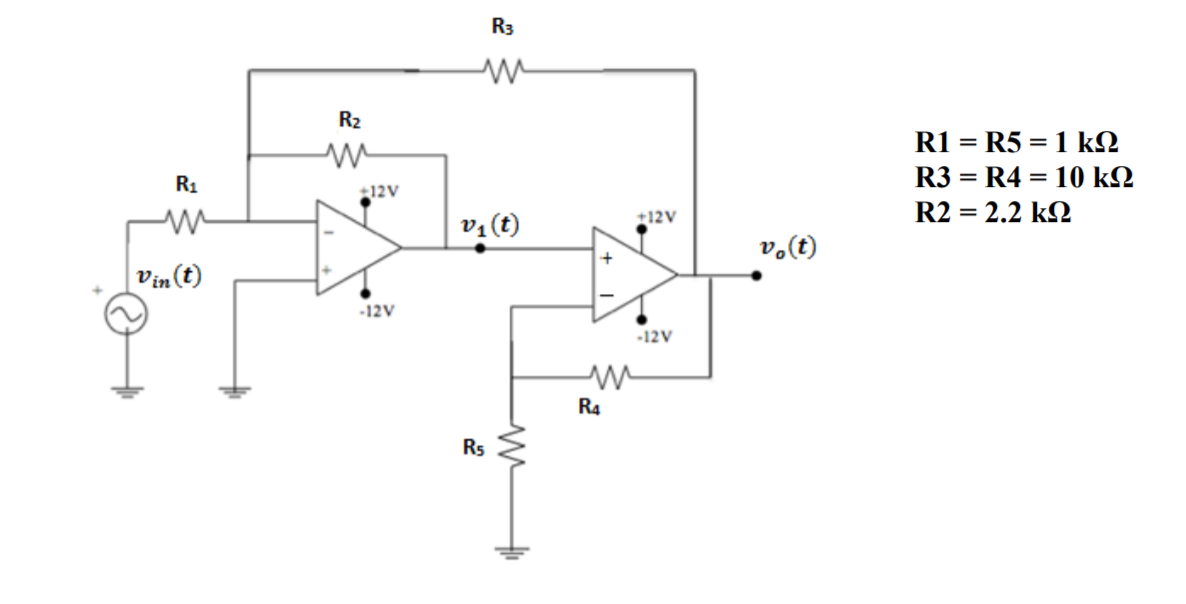
\includegraphics[width=1\textwidth]{circuit_1.png}
   \caption{Circuit schematic for Step 1}
\end{figure}

\subsubsection{a)}
In the circuit given in Figure 1 , \(V_{in}\) is selected as \(0.4sin(1000\pi)\) V. Then, \(V_{out}\) versus \(V_{in}\) characteristic is plotted and shown in Figure 2. 

\begin{figure}[H]
	\centering
   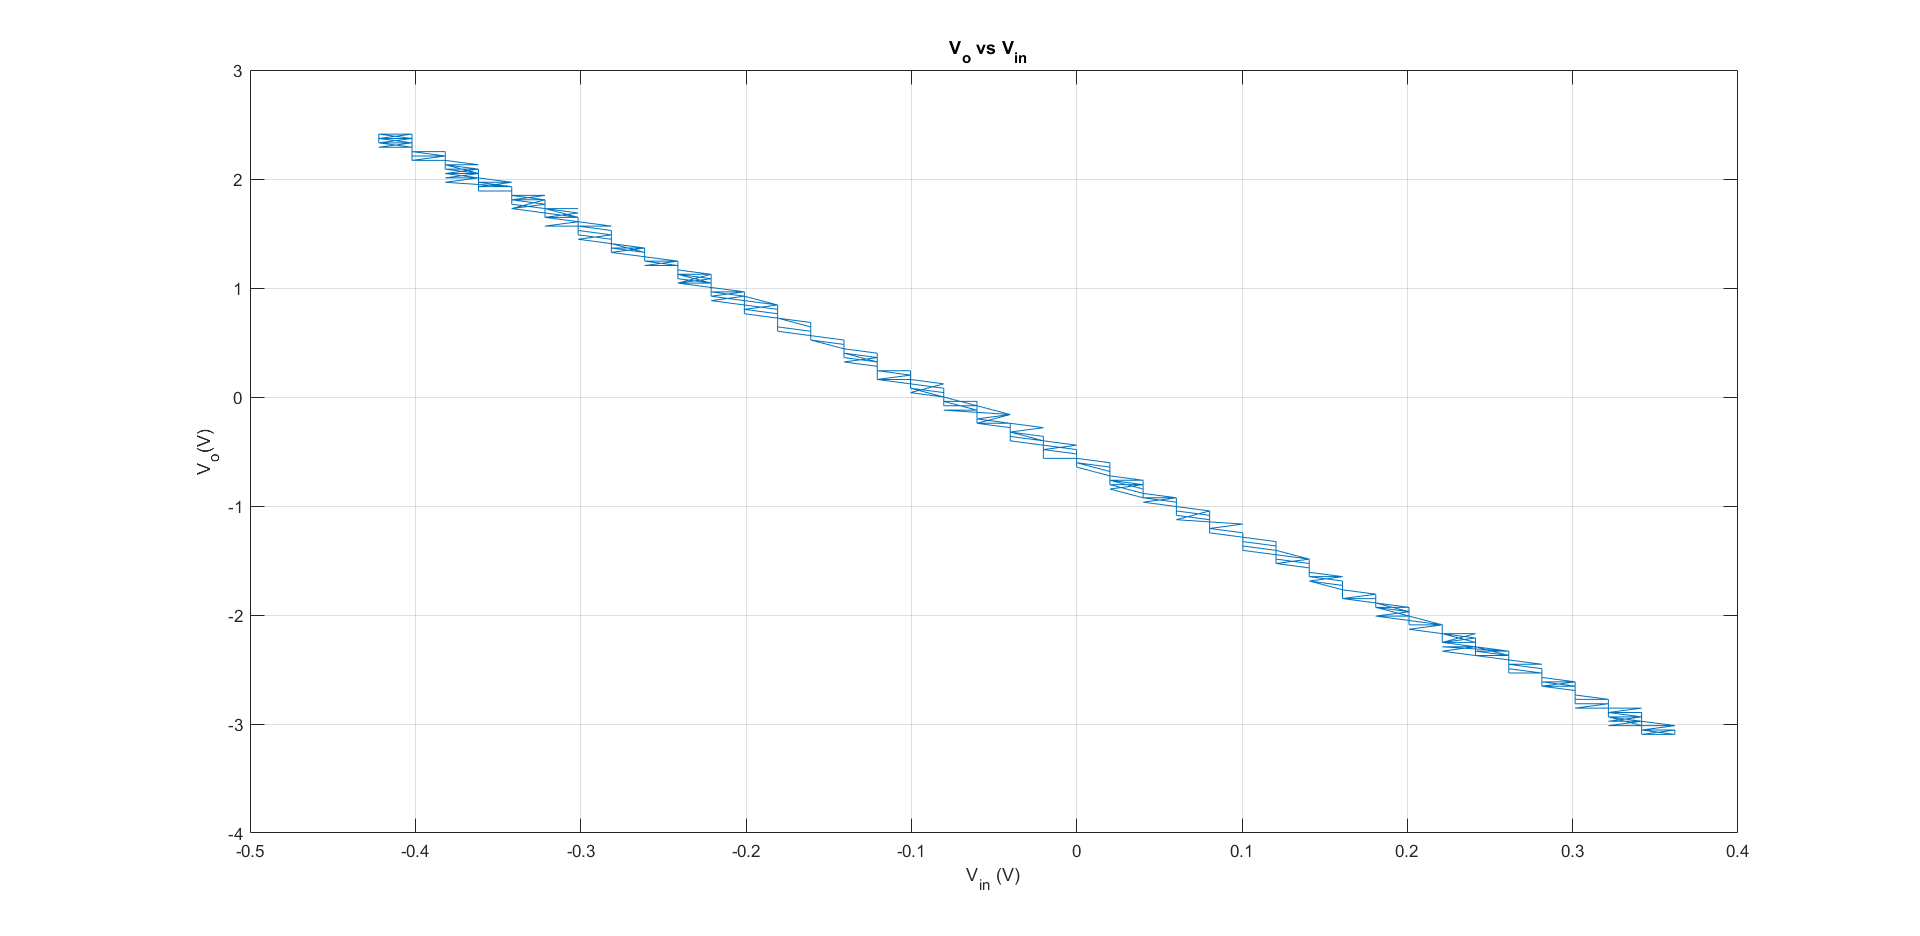
\includegraphics[width=1\textwidth]{1a_1.png}
   \caption{\(V_{o}\) vs \(V_{in}\)}
\end{figure}
The \(V_o\) , \(V_{in}\) waveforms are observed and plotted in MATLAB shown in Figure 3.
\begin{figure}[H]
	\centering
   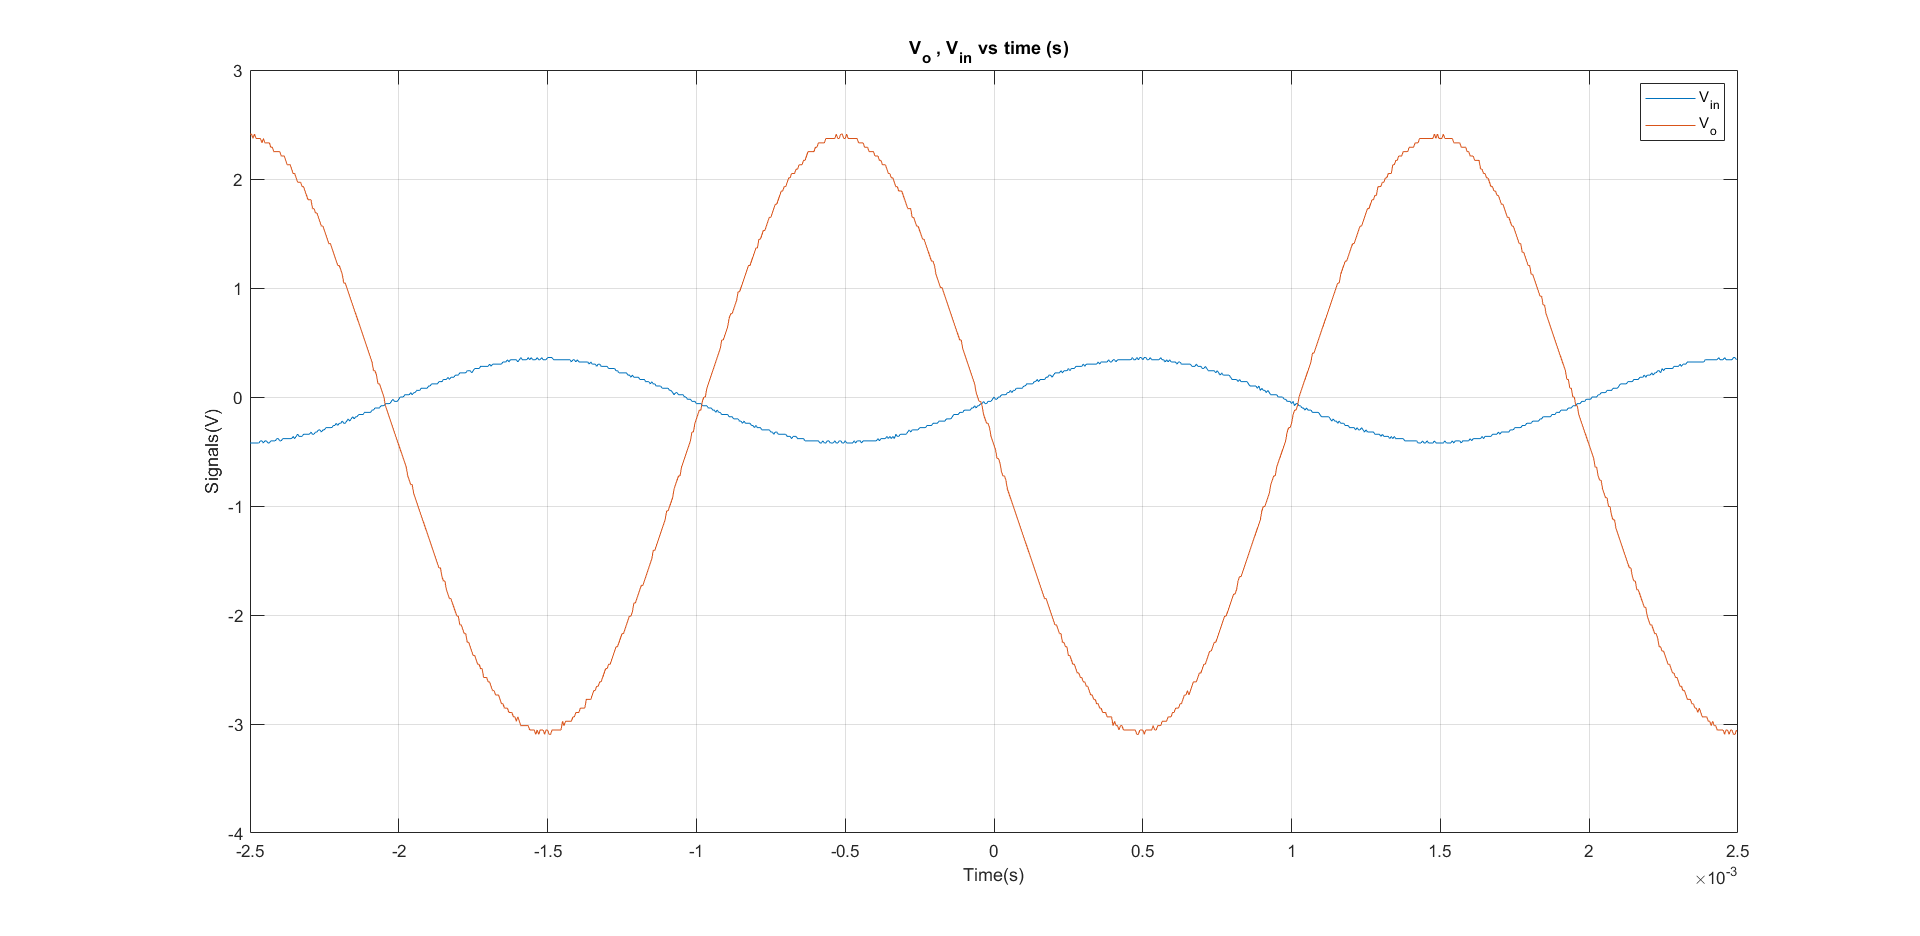
\includegraphics[width=1\textwidth]{1a_2.png}
   \caption{\(V_{o}\) , \(V_{in}\) vs time (s) }
\end{figure}
It can be said that this circuit stays in the linear region with this setup. The input signal is inverted and amplified. In this setup, one inverting and one non-inverting amplifier circuit are combined. So the output is inverting. 
\paragraph{Comparison with the simulation results}
 \mbox{}
\\
The simulation is run in preliminary work according to the circuit shown in Figure 4.
\begin{figure}[H]
	\centering
   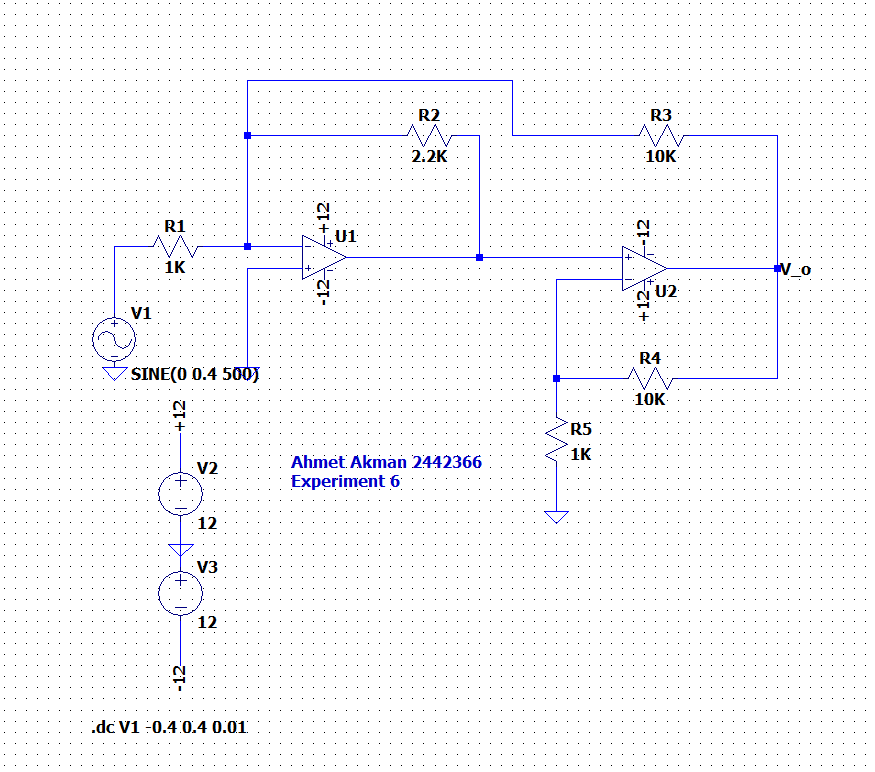
\includegraphics[width=1\textwidth]{Pre1.png}
   \caption{LTSpice schematic for the simulation 1a }
\end{figure}
Then the plot given in Figure 5 is obtained.
\begin{figure}[H]
	\centering
   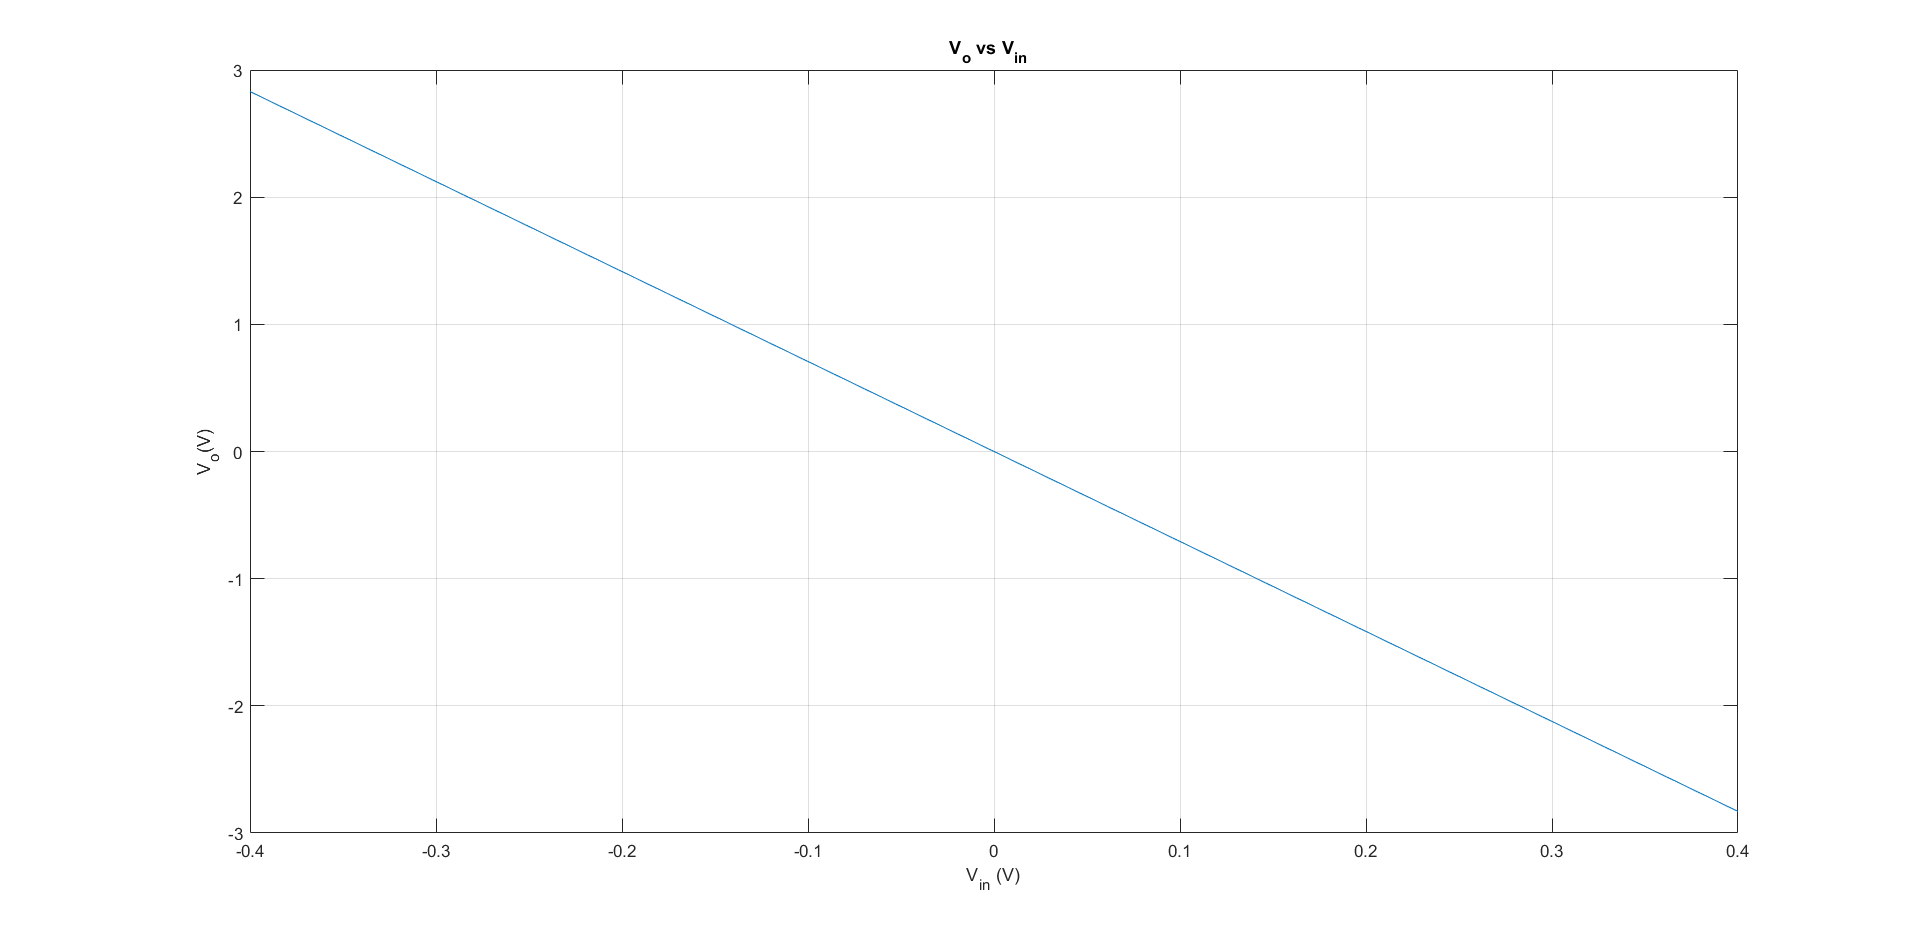
\includegraphics[width=1\textwidth]{Pre_1a.png}
   \caption{\(V_{o}\) vs \(V_{in}\)}
\end{figure}
So, it can be concluded that the theoretical result obtained in preliminary work is quite consistent with the simulation and real-world data. The expression relating \(V_o\) and \(V_in\) is;
\[V_{in} = V_o(\frac{-1}{10} + \frac{-5}{121})\]
There is a slight offset of signal in the actual plot. This is predicted to be stemmed from the non-ideality of either the LM741 component or the power line of the power supply.


\subsubsection{b)}
In the circuit given in Figure 1 , \(V_{in}\) is kept as \(0.4sin(1000\pi)\) V. Then \(R3\) is removed from the circuit. The \(V_{out}\) versus \(V_{in}\) characteristic is plotted and shown in Figure 6. 


\begin{figure}[H]
	\centering
   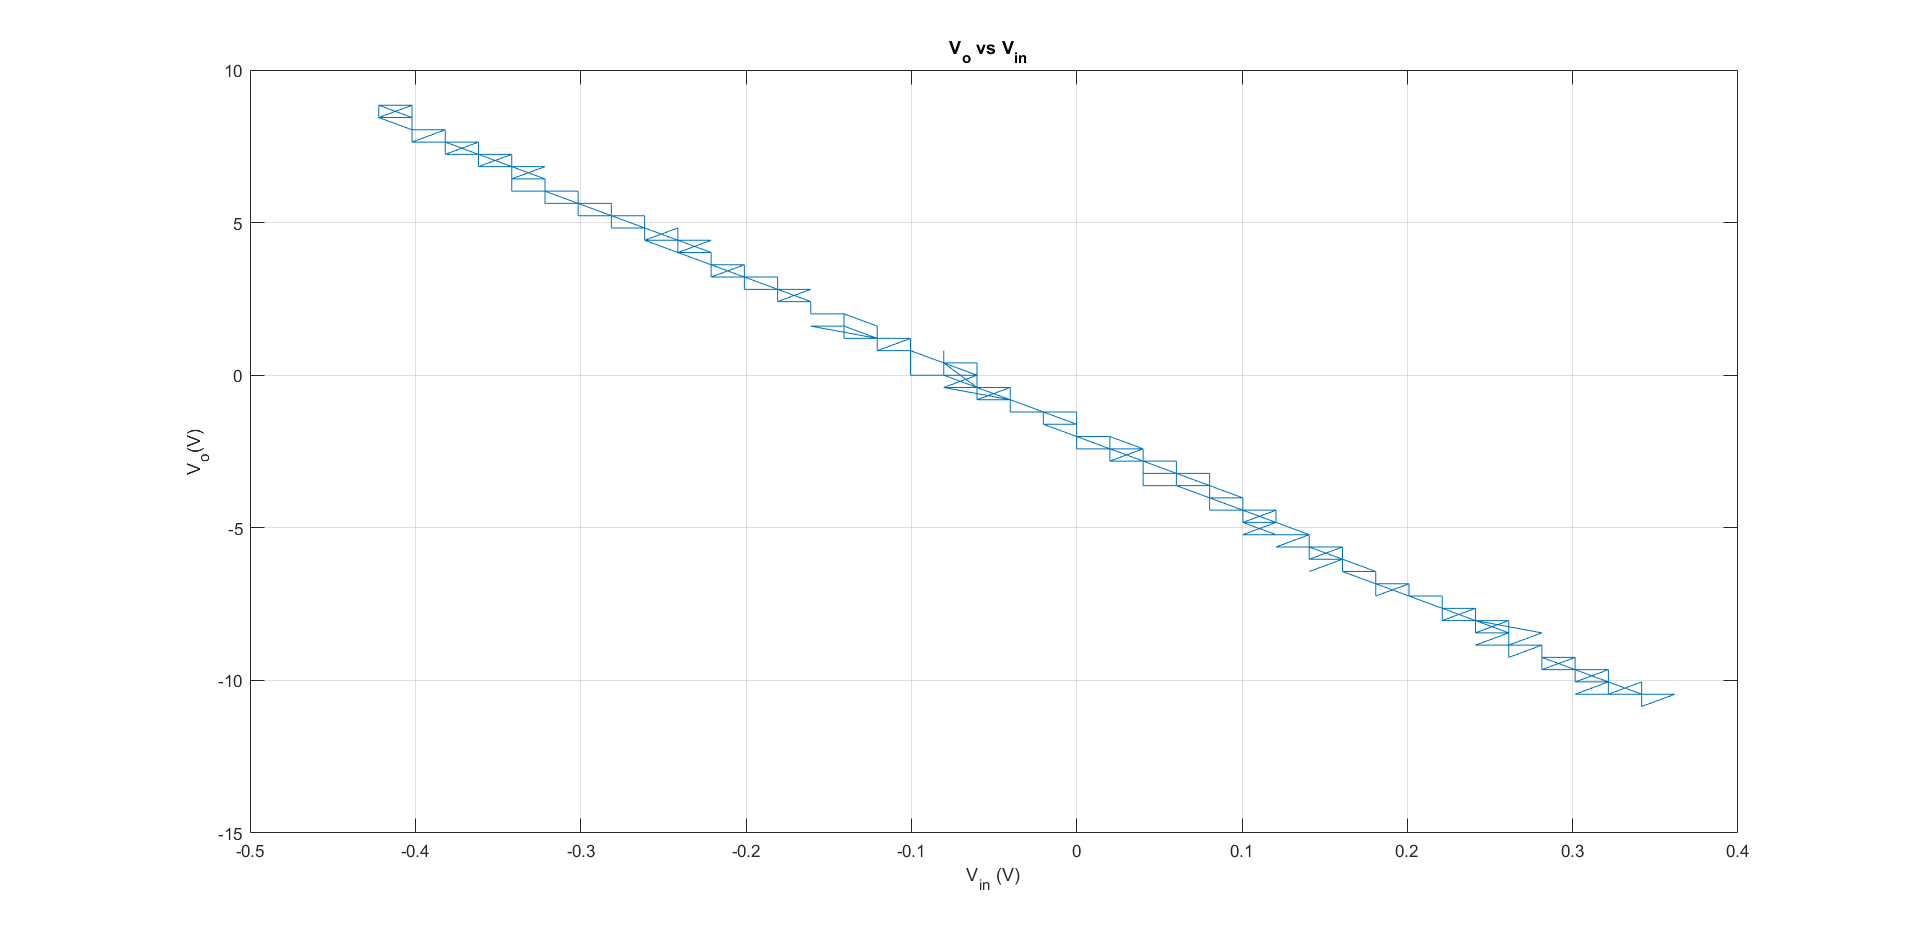
\includegraphics[width=1\textwidth]{1b_1.png}
   \caption{\(V_{o}\) vs \(V_{in}\)}
\end{figure}
The \(V_o\) , \(V_{in}\) waveforms are also observed and plotted in MATLAB shown in Figure 7.
\begin{figure}[H]
	\centering
   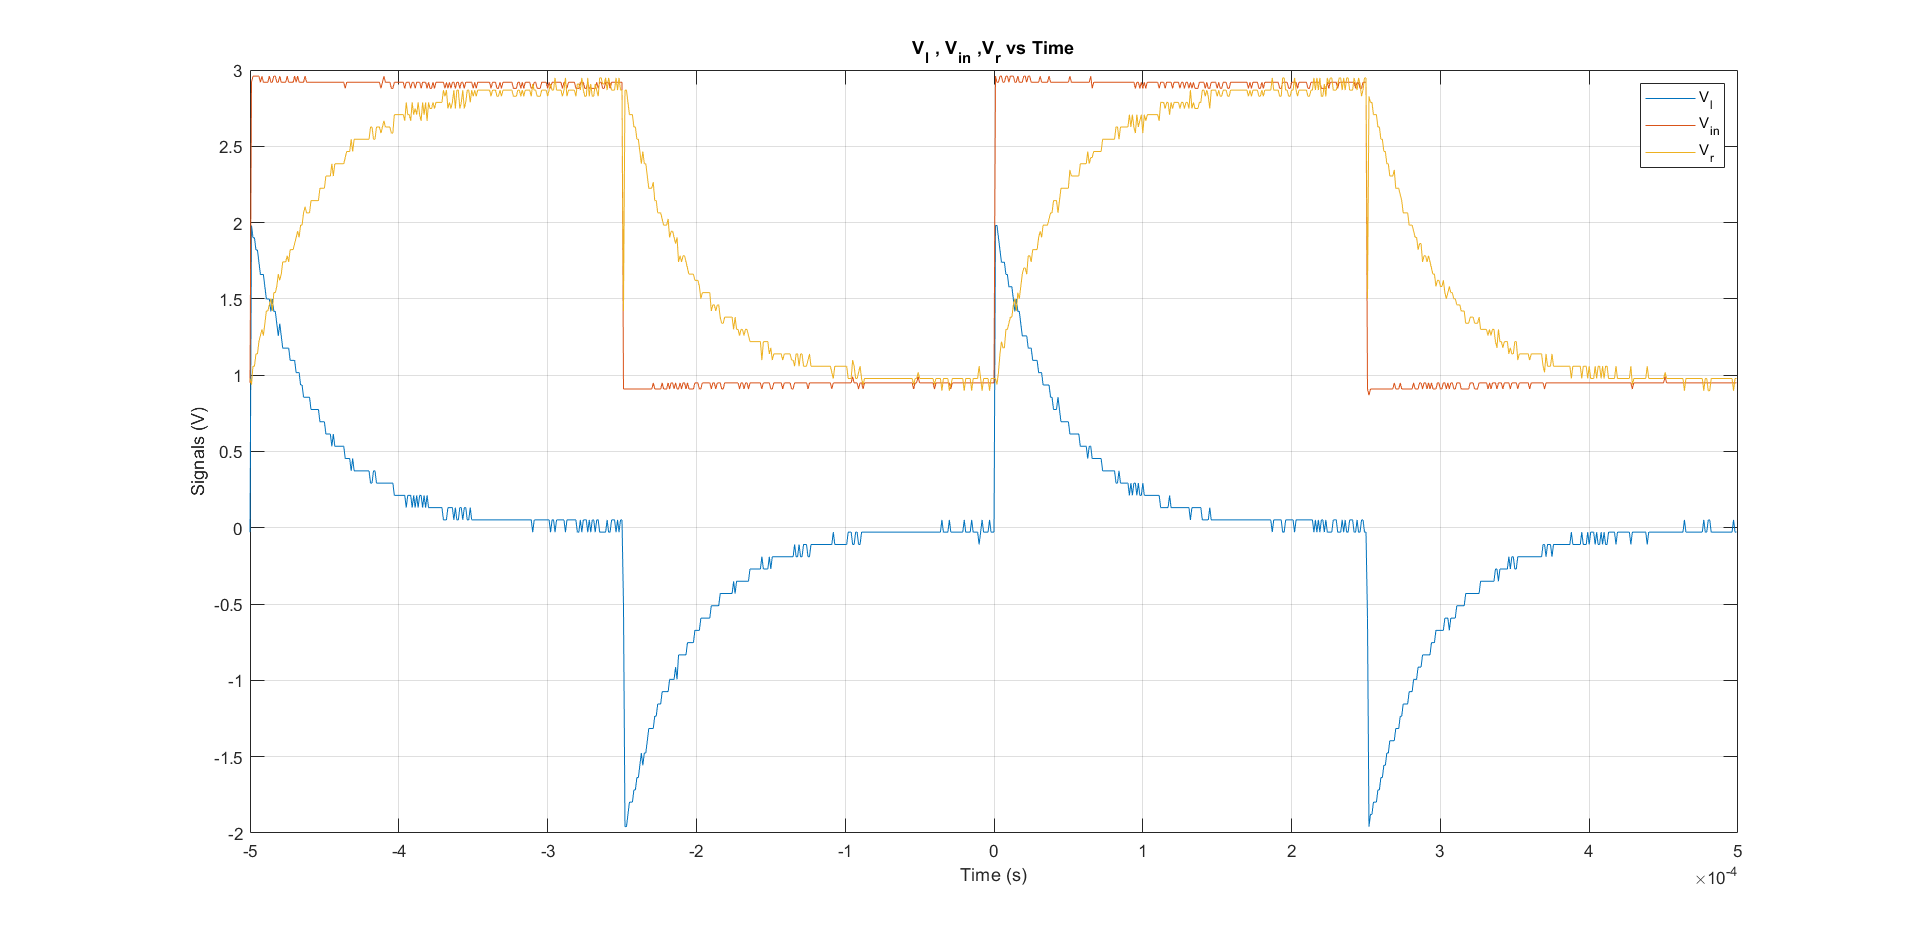
\includegraphics[width=1\textwidth]{1b_2.png}
   \caption{\(V_{o}\) , \(V_{in}\) vs time (s) }
\end{figure}
It can be stated that in this configuration, the first opamp is not propagated with negative feedback from the \(V_o\), so the signal is amplified more.  
\paragraph{Comparison with the simulation results}
 \mbox{}
\\
The simulation is run in preliminary work according to the circuit shown in Figure 4 by removing the R3 connection. So the \(V_{o}\) vs \(V_{in}\) result is shown in Figure 8.
\begin{figure}[H]
	\centering
   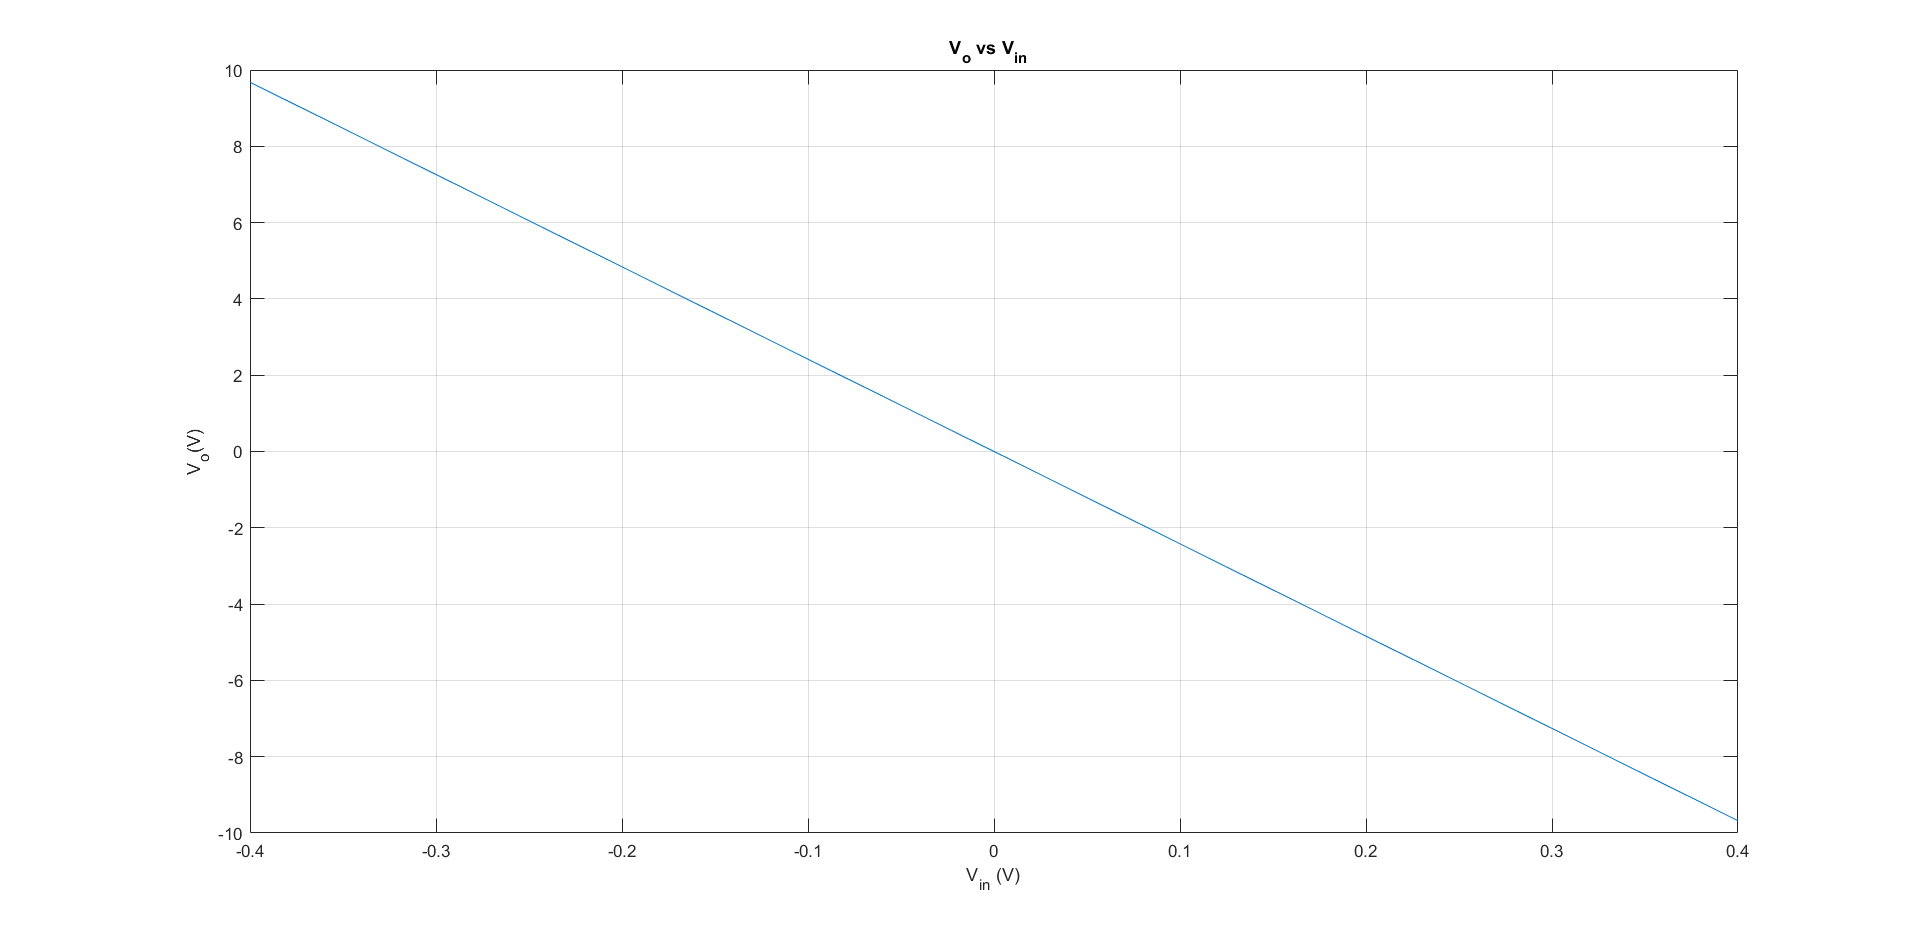
\includegraphics[width=1\textwidth]{Pre_1b.png}
   \caption{\(V_{o}\) vs \(V_{in}\)}
\end{figure}
It can be concluded that the laboratory results and simulation results are quite consistent. The relation found in preliminary work seems to behold which is;
\[V_{in} = \frac{-5 V_o}{121} \]
Also, there is a shift towards the negative side in the laboratory plot. This is predicted to be sourced from the non-ideality of either the LM741 component or the power line of the power supply.
\subsubsection{c)}
The circuit setup is conserved in this section. The \(V_{in}\) is selected as \(1sin(200\pi)\) V this time. \(V_{o}\) vs \(V_{in}\) is obtained as shown in Figure 9.
\begin{figure}[H]
	\centering
   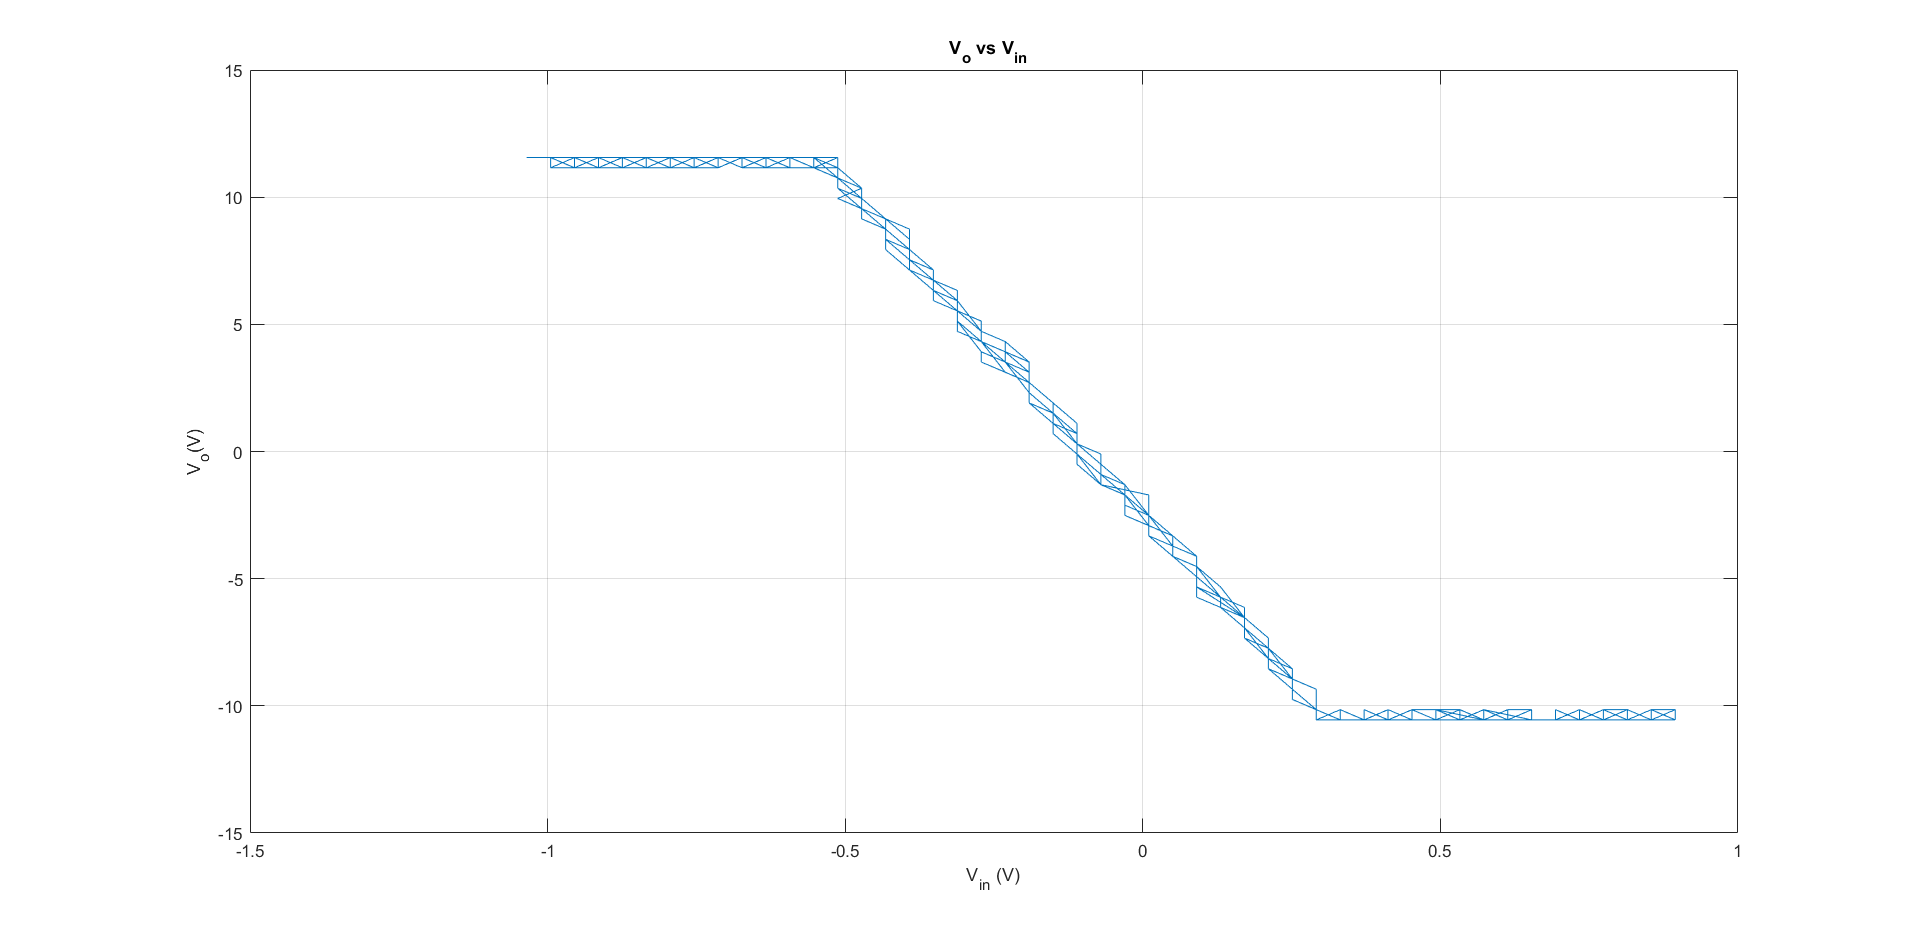
\includegraphics[width=1\textwidth]{1c_1.png}
   \caption{\(V_{o}\) vs \(V_{in}\)}
\end{figure}
The waveforms \(V_0\) and \(V_{in}\) are observed and plotted in the time domain is given in Figure 10.
\begin{figure}[H]
	\centering
   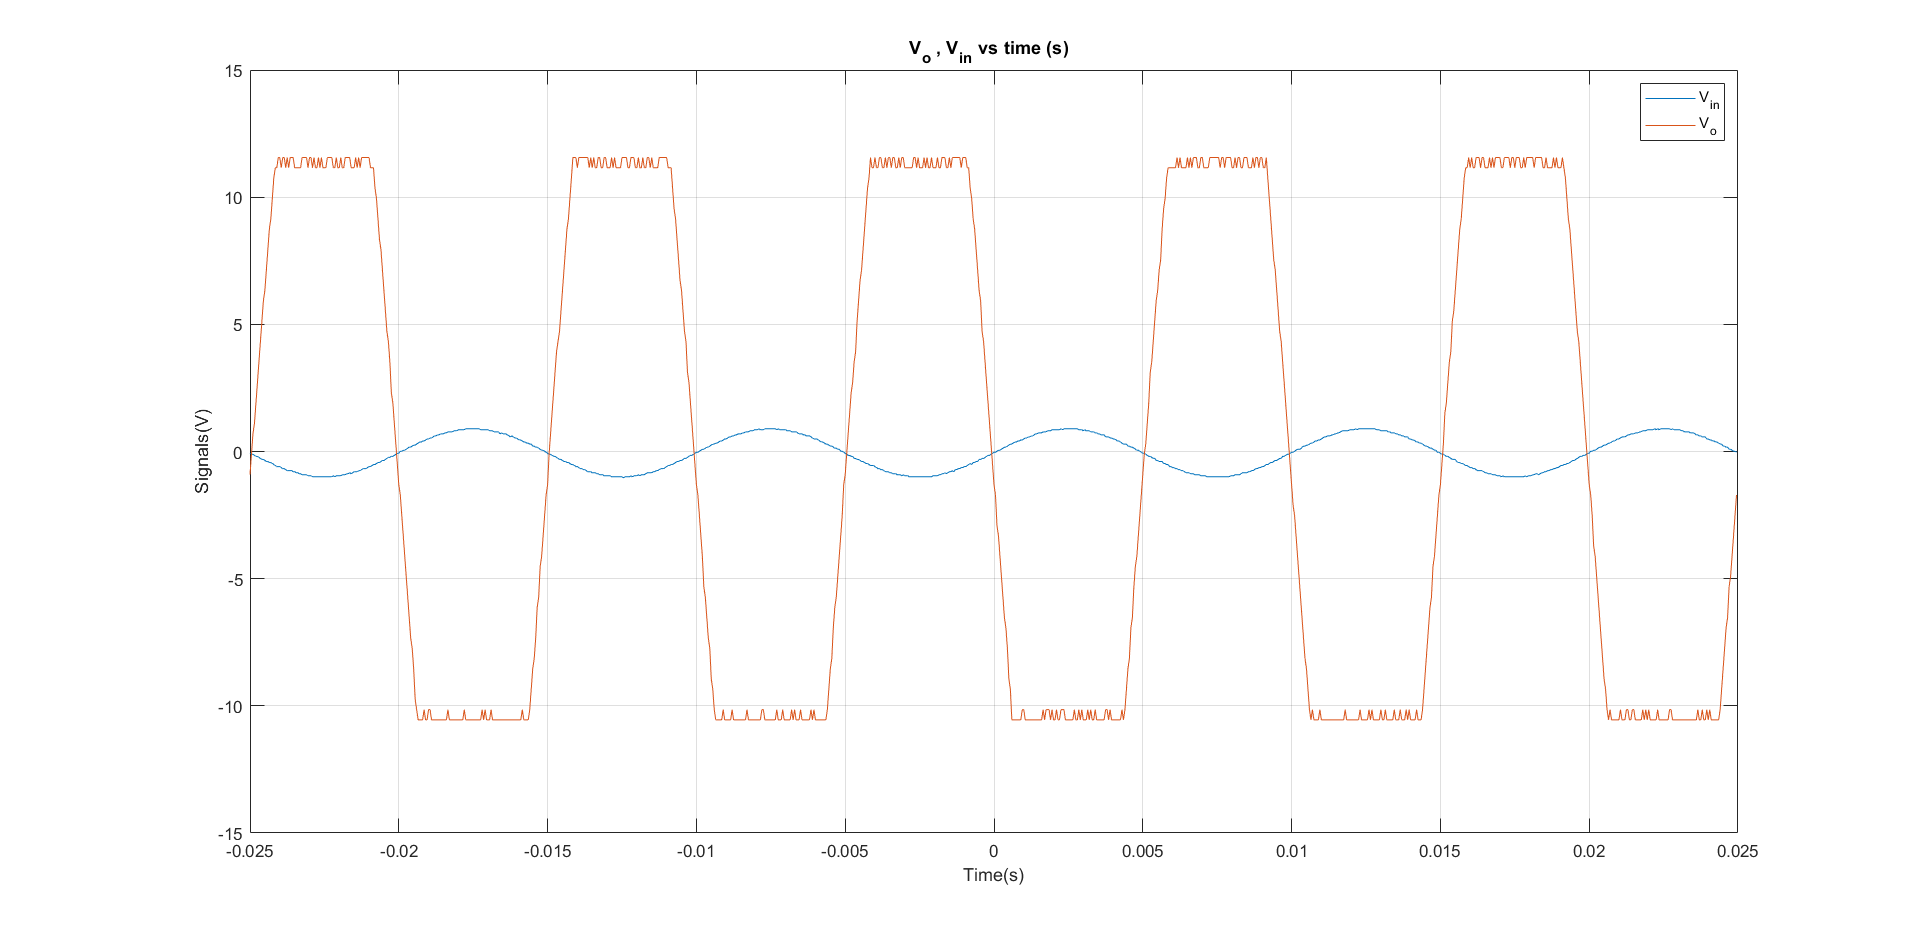
\includegraphics[width=1\textwidth]{1c_2.png}
   \caption{\(V_{o}\) , \(V_{in}\) vs time (s) }
\end{figure}
As a result, it can be stated that when the signal amplitude increases, the opamp(s) may not stay at their linear region can be saturated. This circuit setup, in principle, always amplifies the signal and inverts it.
\subsection{Step 2}
In this step the non-linear inverting amplifier circuit given in Figure 11 is set. The \(V_{in}\) is set to \(3sin(200\pi t)\).
\begin{figure}[H]
	\centering
   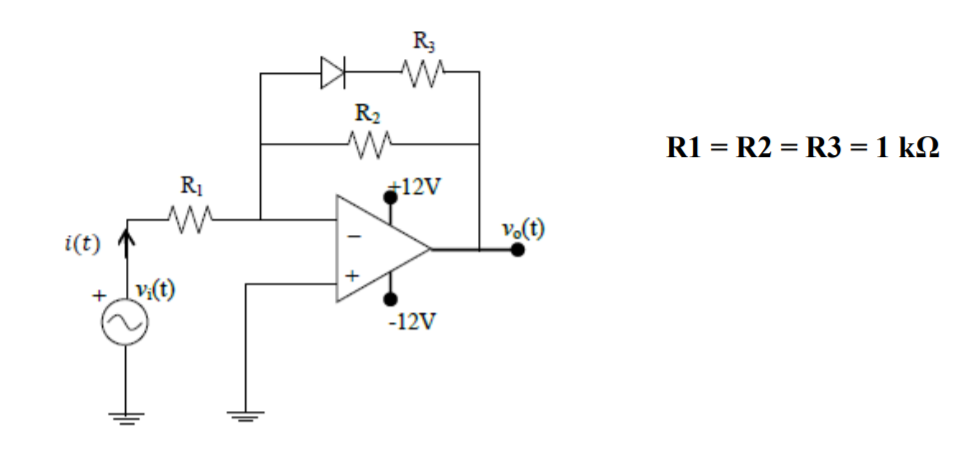
\includegraphics[width=1\textwidth]{circuit_2.png}
   \caption{Circuit schematic for Step 2}
\end{figure}
The \(V_{o}\) versus \(V_{in}\) data is plotted and shown in Figure 12. 

\begin{figure}[H]
	\centering
   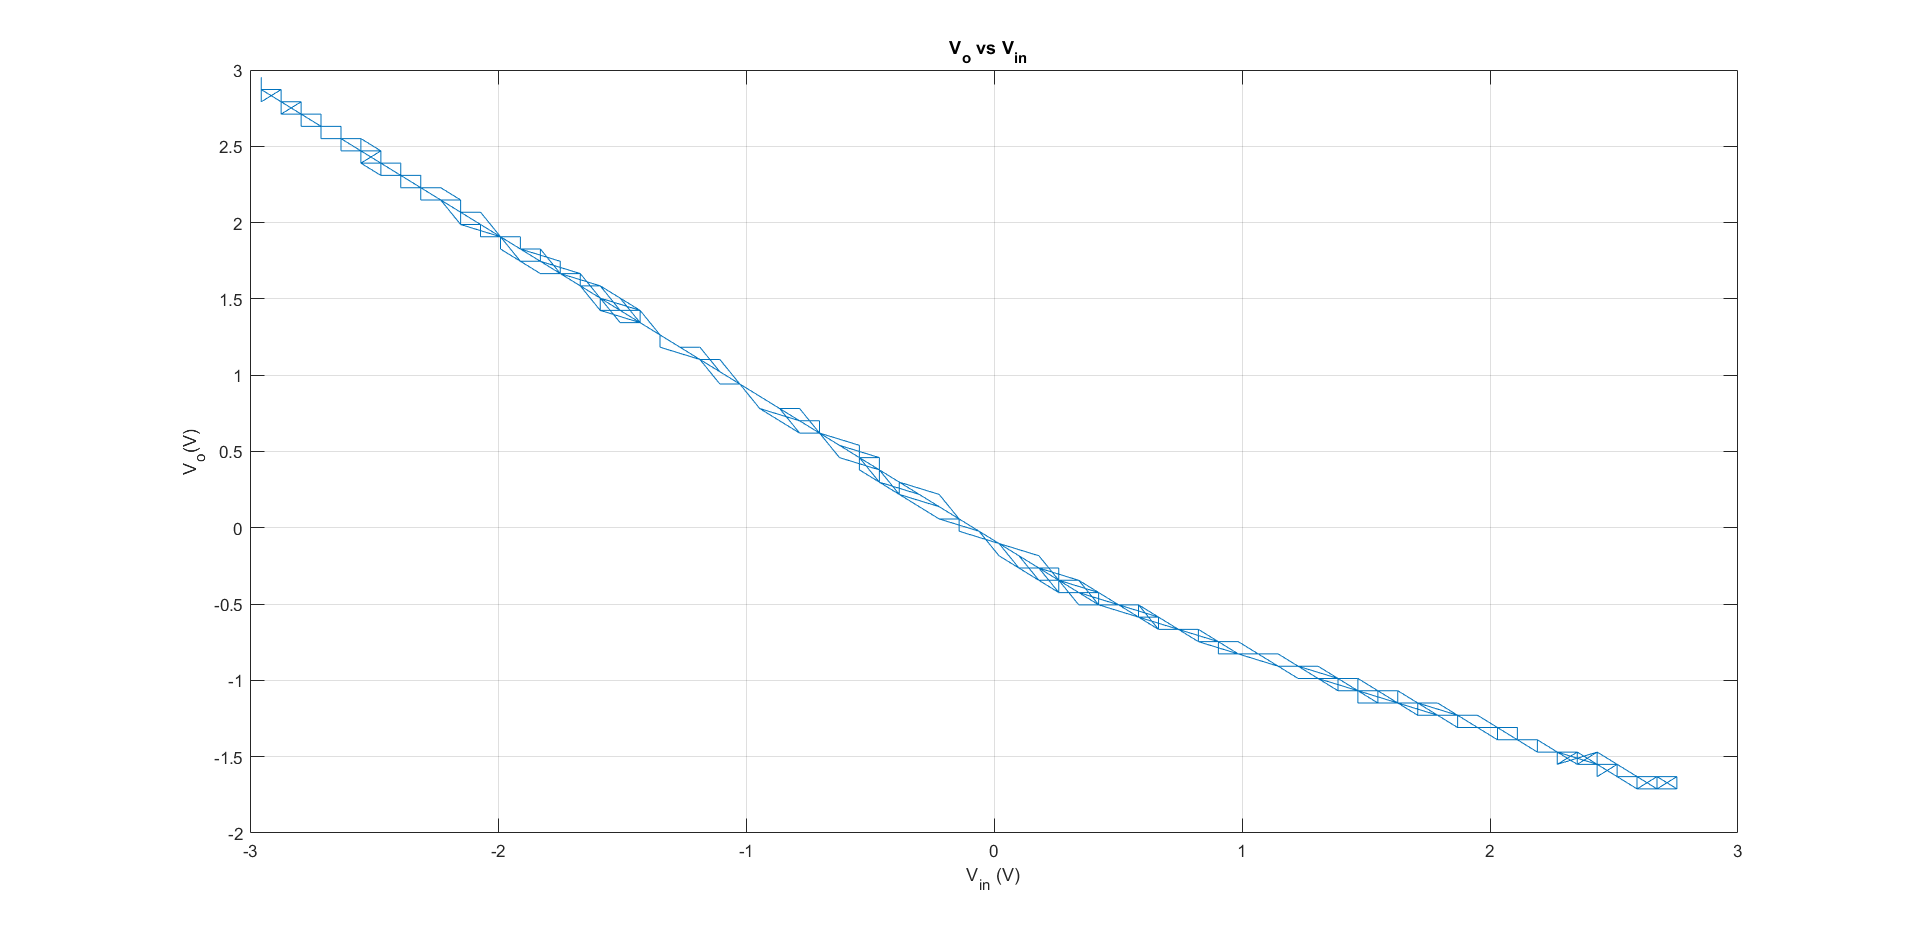
\includegraphics[width=1\textwidth]{2_1.png}
   \caption{\(V_{o}\) vs \(V_{in}\)}
\end{figure}
The waveforms \(V_{o}\) and \(V_{in}\) are plotted in the same graph given in Figure 13.
\begin{figure}[H]
	\centering
   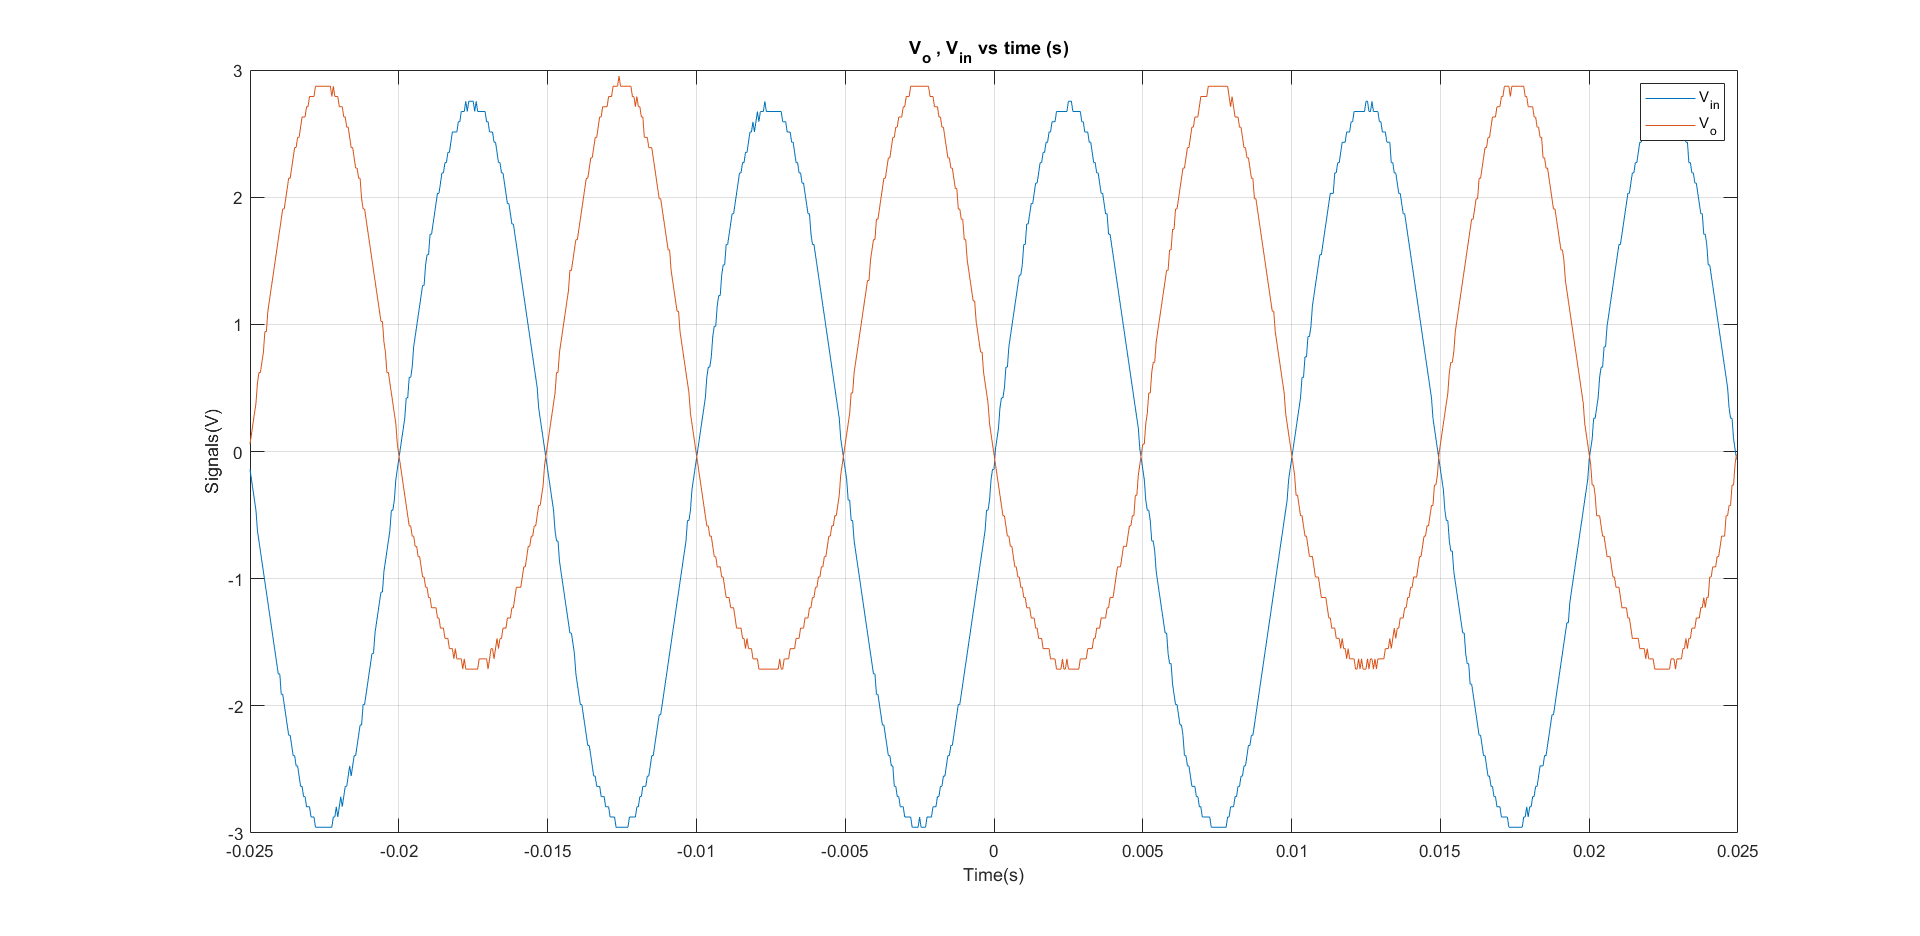
\includegraphics[width=1\textwidth]{2_2.png}
   \caption{\(V_{o}\) , \(V_{in}\) vs time (s) }
\end{figure}
As a result, the comment can be made such that the amplifier stays in the linear region ,and when the diode is on negative feedback, resistance is lower than the situation diode is off. So, the slopes of the negative and positive areas are different.
\subsubsection{Comparison with the simulation results}
The circuit given in Figure 14 is constructed in LTSpice environment.
\begin{figure}[H]
	\centering
   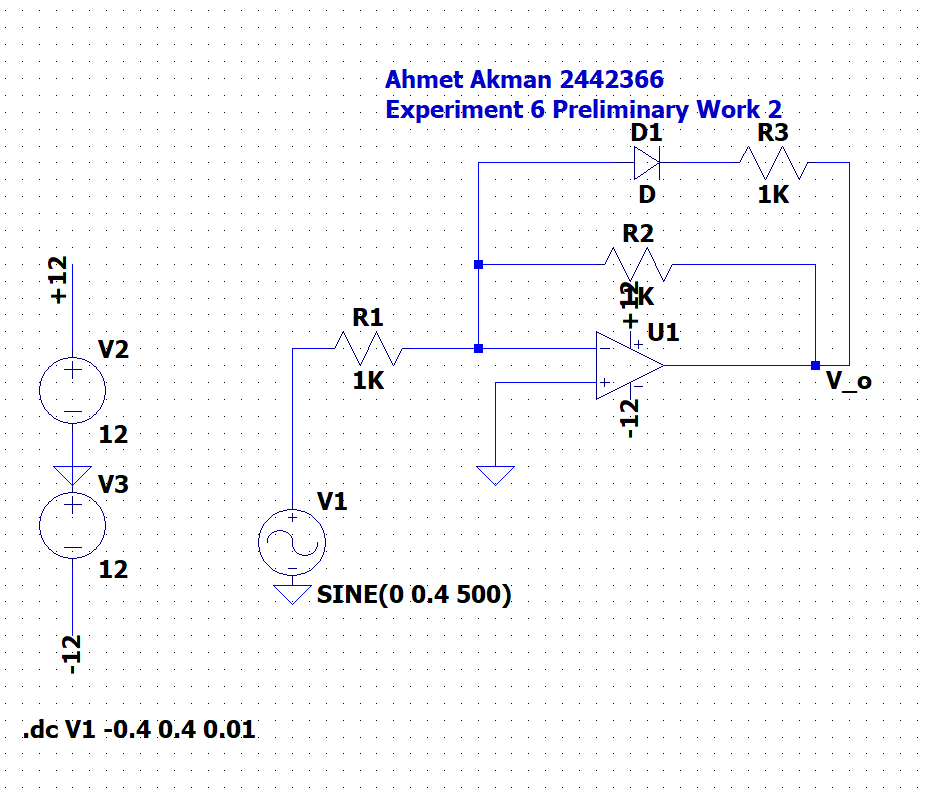
\includegraphics[width=1\textwidth]{Pre2.png}
   \caption{LTSpice schematic for the simulation 2 }
\end{figure}
Then \(V_{o}\) versus \(V_{in}\) is obtained and shown in Figure 15. 
\begin{figure}[H]
	\centering
   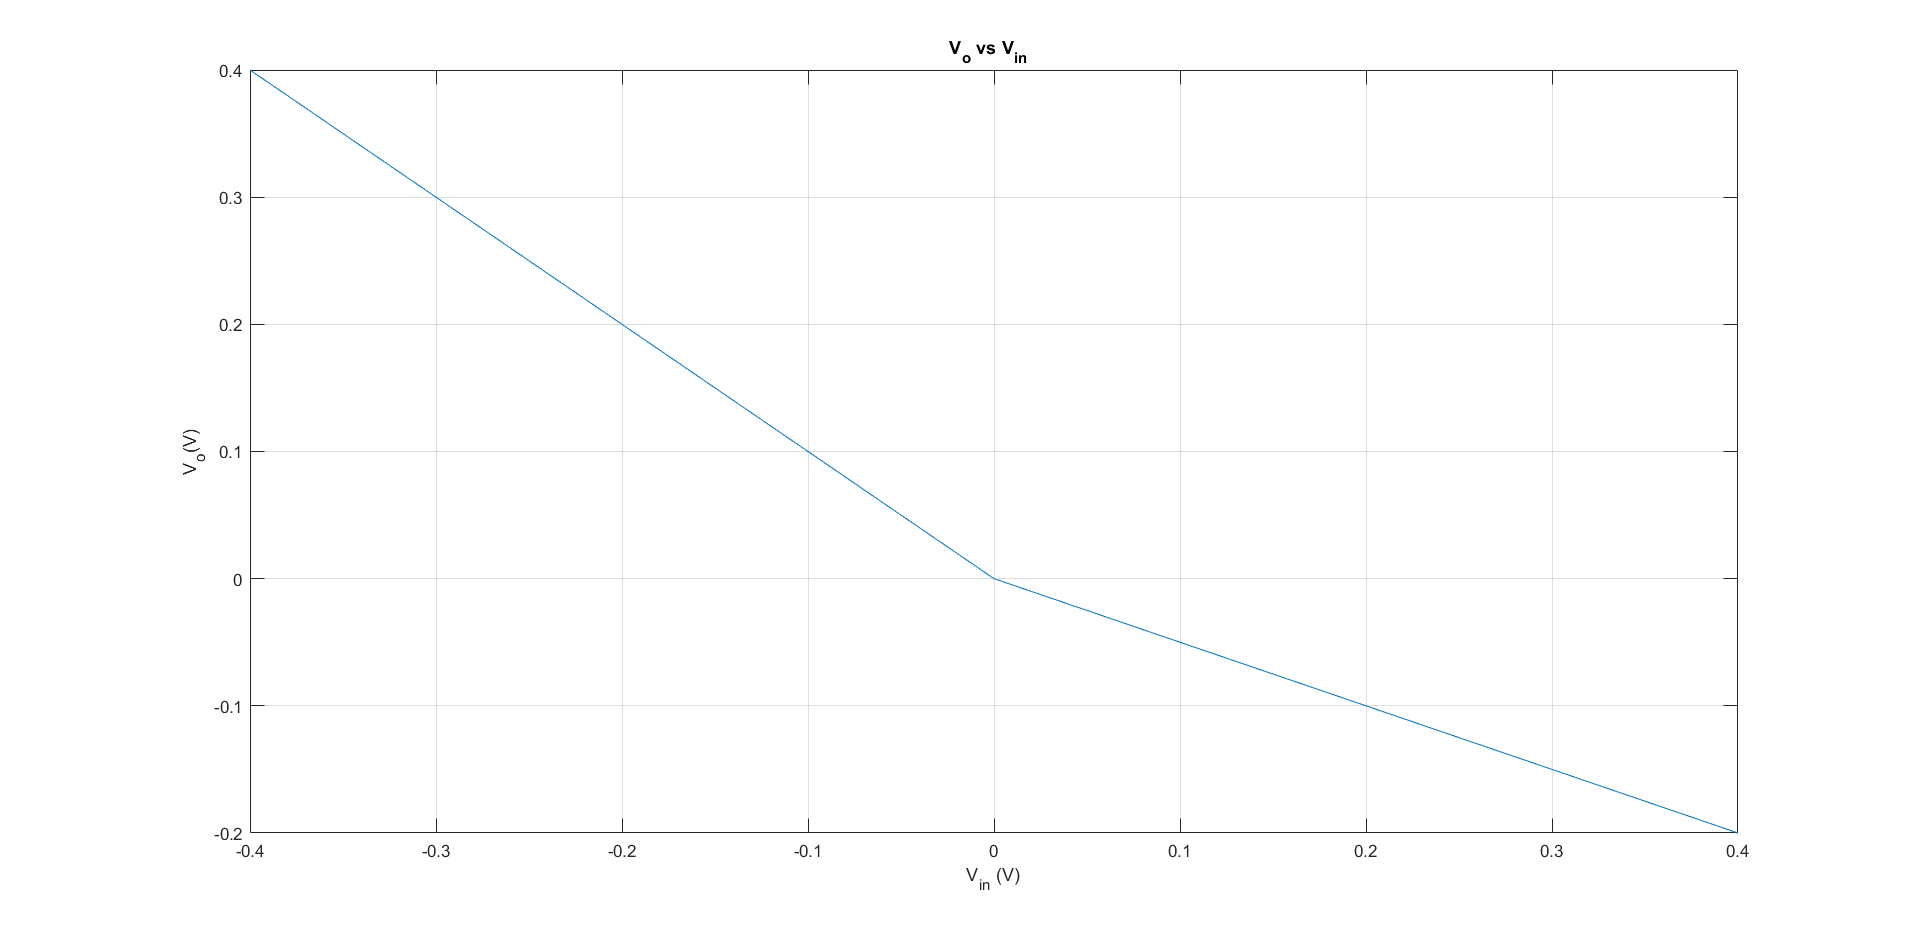
\includegraphics[width=1\textwidth]{Pre_2.png}
   \caption{\(V_{o}\) vs \(V_{in}\)}
\end{figure}
It can be concluded that the measurements are consistent with the simulation and the equation obtained in the preliminary work. The equation is,

\begin{center}
if \(V_- > V_o\),  \(-2V_o = V_{in}\) \\
	if \(V_- < V_o\),  \(-V_o = V_{in}\)
\\
\end{center}
So the results are also consistent with the theoretical calculations. Also, there is a shift towards the negative y-axis in the laboratory plot. This is predicted to be sourced from the non-ideality of either the LM741 component or the diode component.
\subsection{Step 3}
In this step, the circuit called negative resistance converter, which is shown in Figure 16, is constructed.  
\begin{figure}[H]
	\centering
   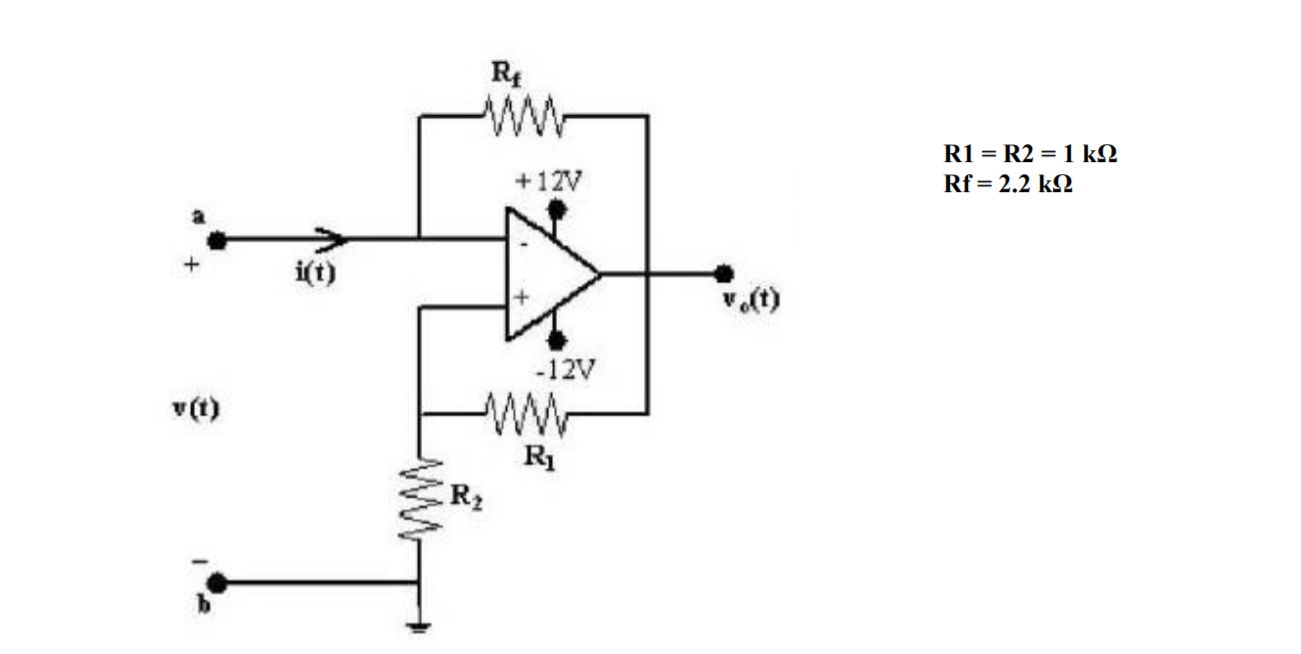
\includegraphics[width=1\textwidth]{circuit_5.png}
   \caption{Circuit schematic for Step 3}
\end{figure}

\subsubsection{a)}
Figure 17 shows the \(V_{o}\) versus \(V_{in}\) characteristic obtained when \(V_{in}= 10sin(200\pi t) \).
\begin{figure}[H]
	\centering
   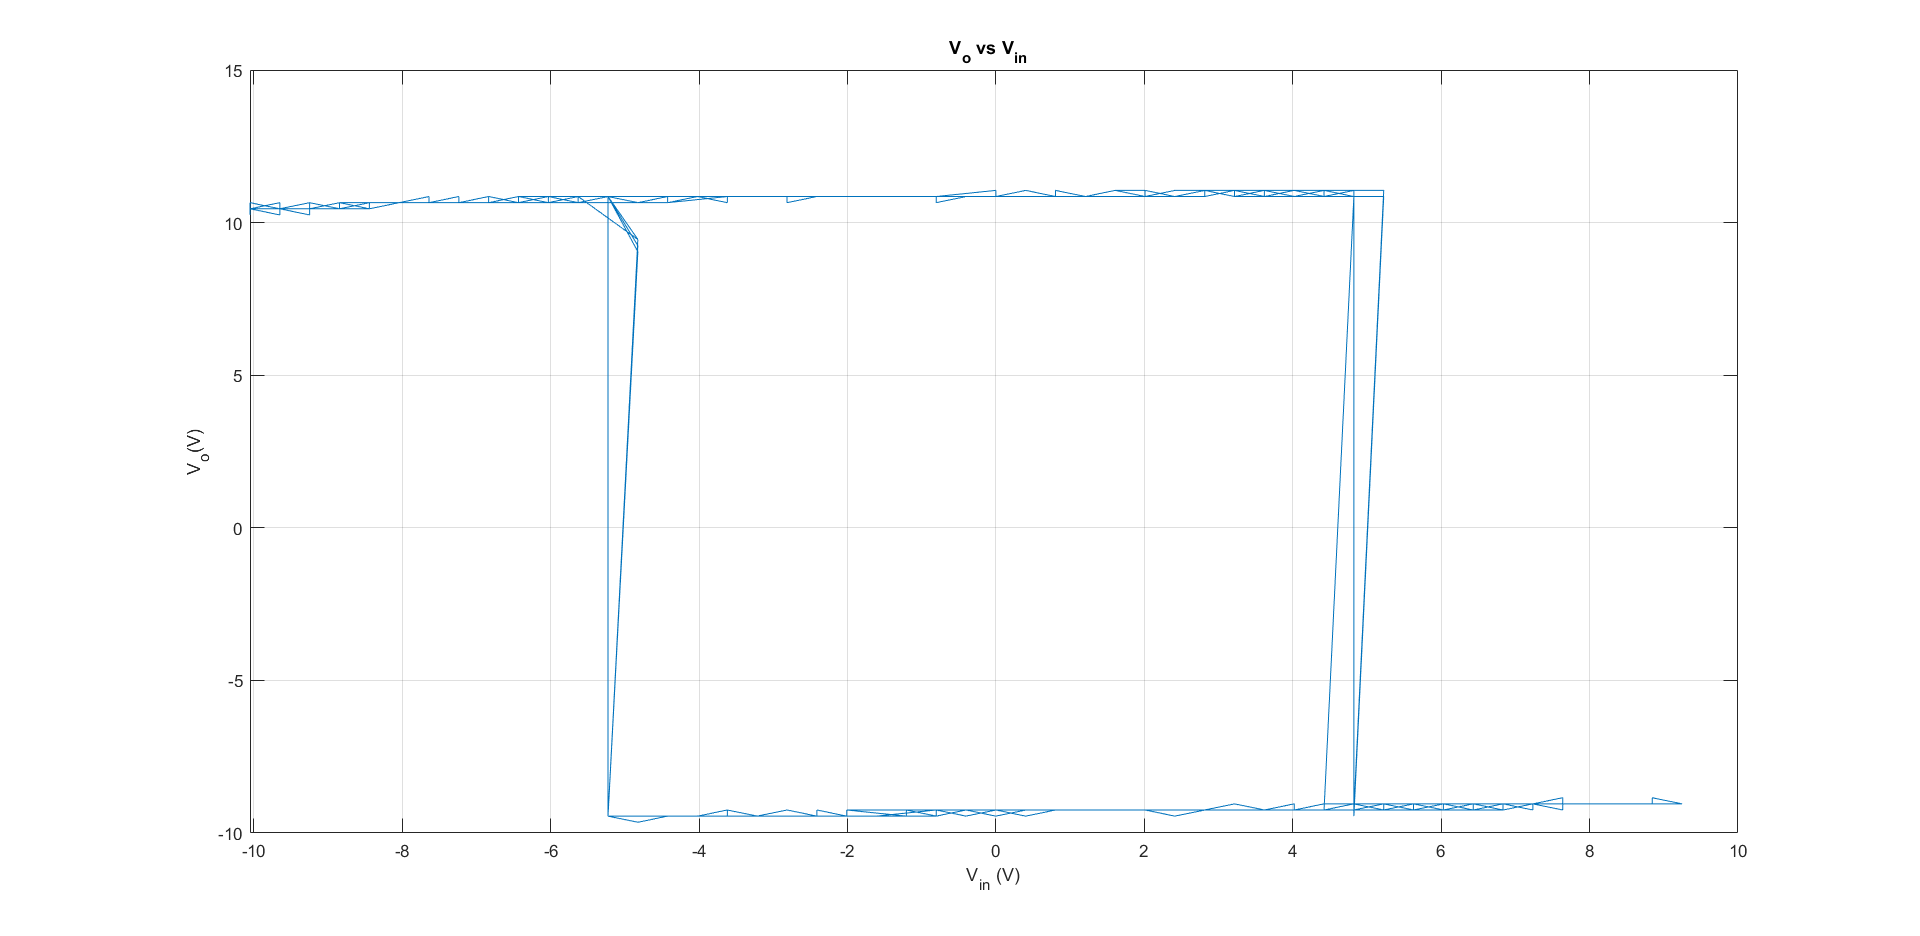
\includegraphics[width=1\textwidth]{3a_1.png}
   \caption{\(V_{o}\) vs \(V_{in}\)}
\end{figure}
In order to plot \(i_{in}\) versus \(V_{in}\) , the same data can be used. If we subtract \(V_{in}\) from \(V_o\) and divide it by \(R_f\) we can get the \(V_{in}\) value and plot it. So the resulting plot is given in Figure 18.

\begin{figure}[H]
	\centering
   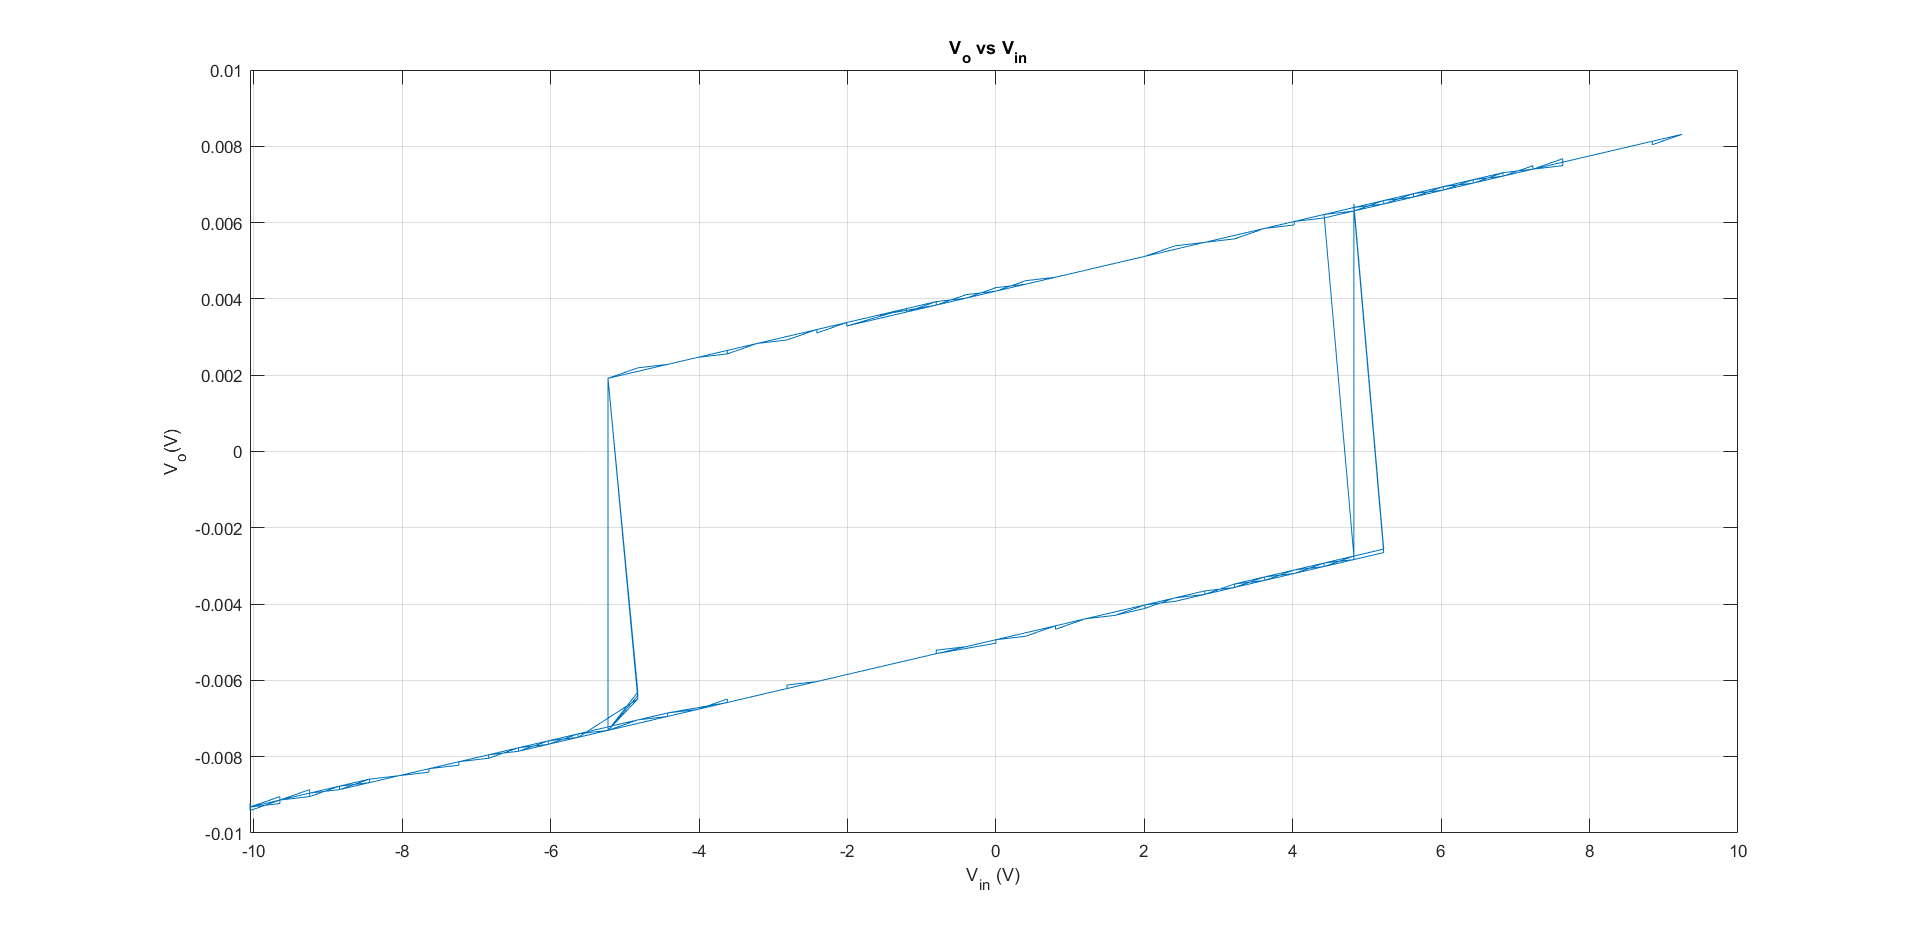
\includegraphics[width=1\textwidth]{3a_1_new.png}
   \caption{\(i_{in}\) vs \(V_{in}\)  }
\end{figure}

In figure 19 the waveforms \(V_{o}\) , \(V_{in}\) plotted against time. 
\begin{figure}[H]
	\centering
   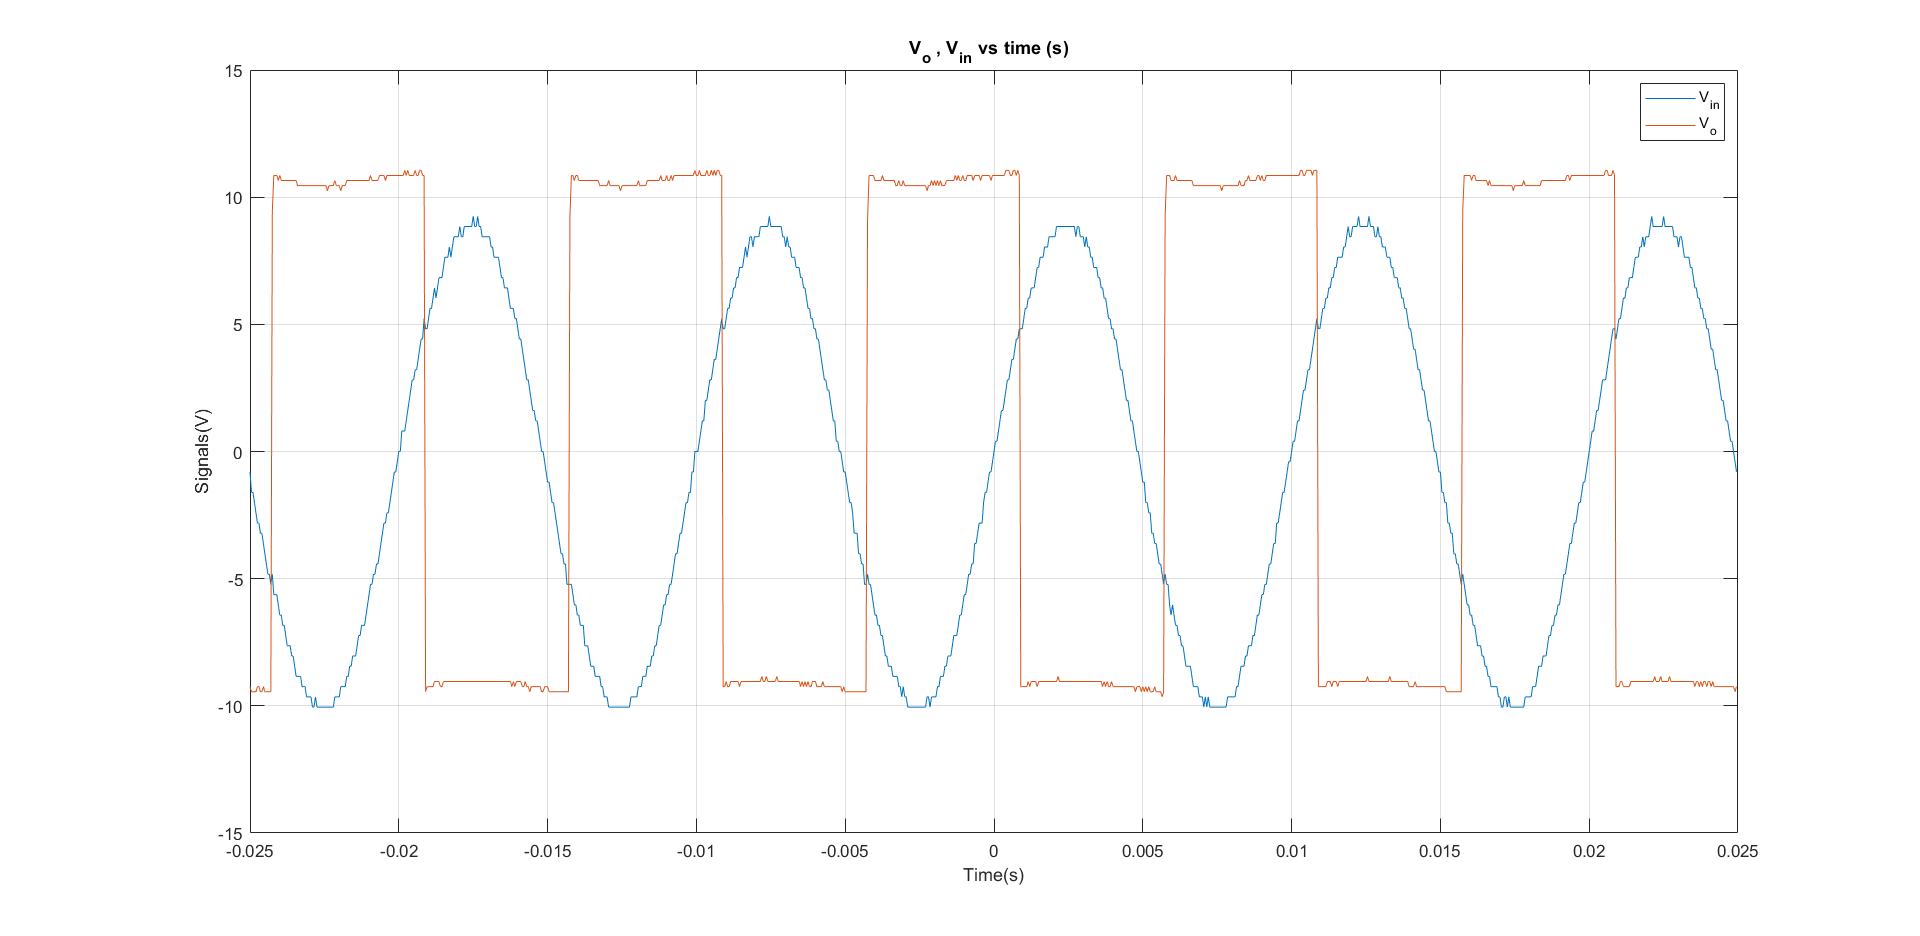
\includegraphics[width=1\textwidth]{3a_2.png}
   \caption{\(V_{o}\) , \(V_{in}\) vs time (s) }
\end{figure}


\subsubsection{b)}
In this part, the circuit setup is conserved except for signal generator input. A 1 \(\mu F\) capacitor is connected across the terminals a and b.  
The data of capacitor voltage \(V_c\) and output voltage \(V_o\) is obtained and plotted, which is shown in Figure 20. 
\begin{figure}[H]
	\centering
   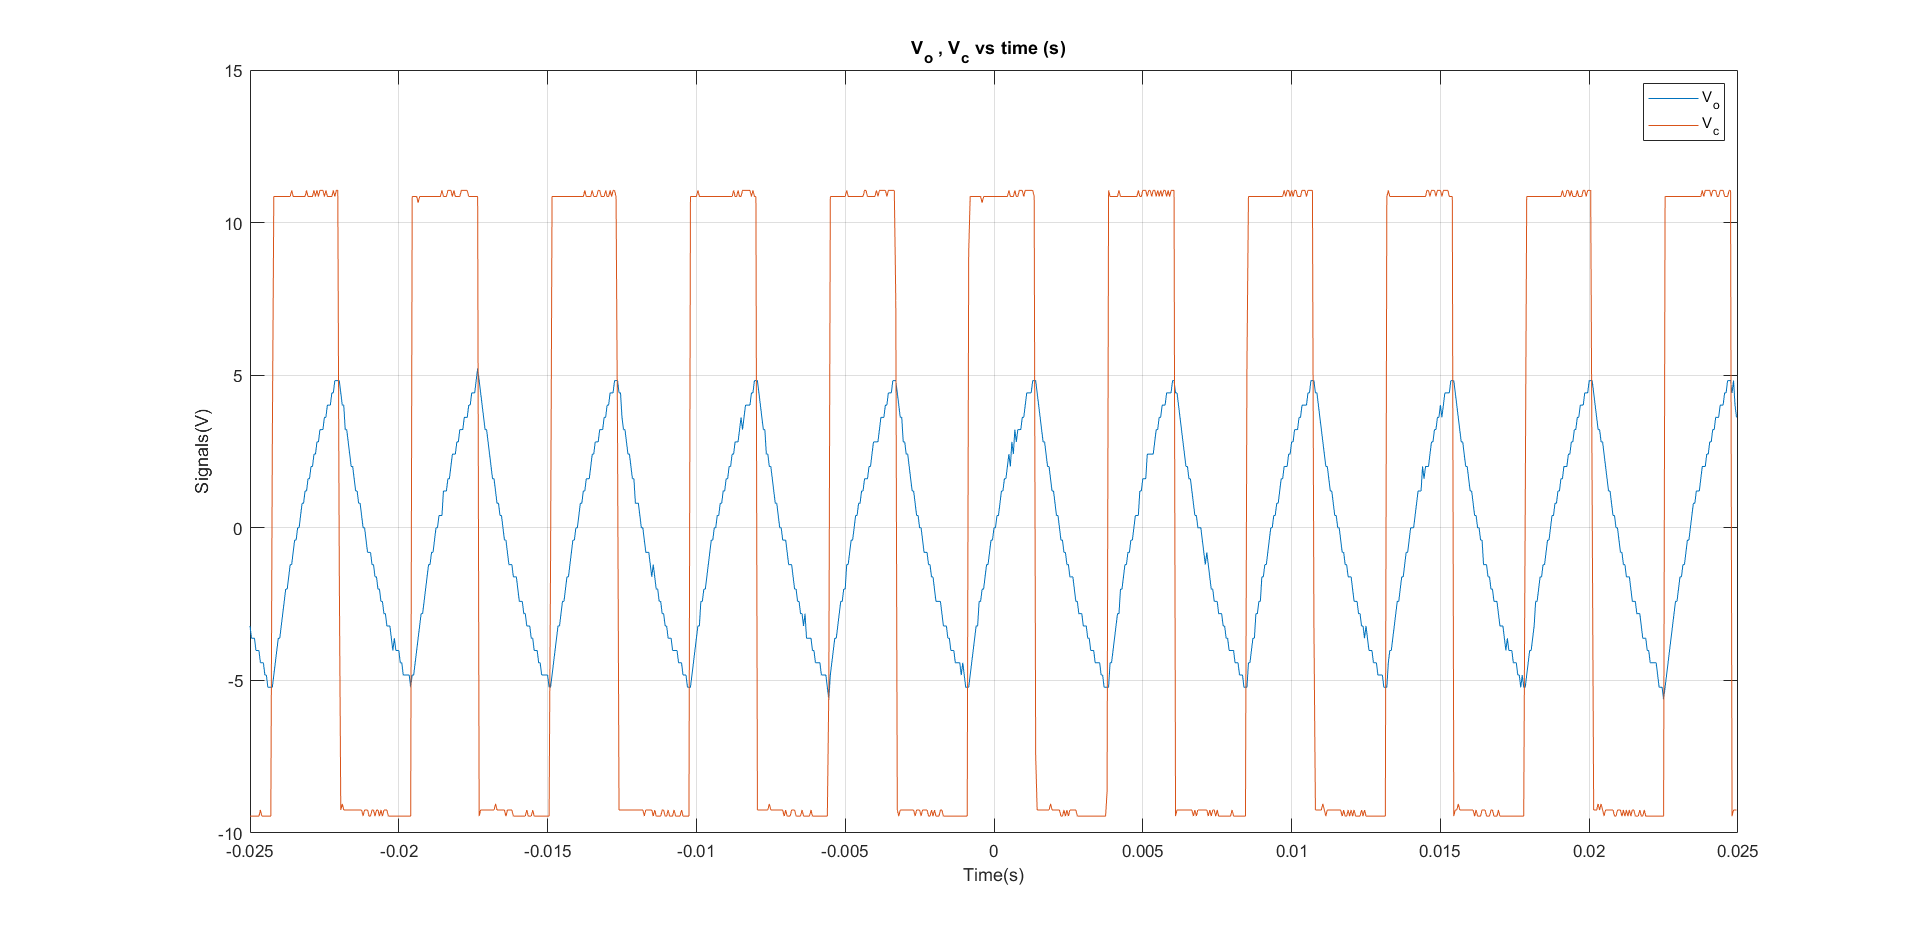
\includegraphics[width=1\textwidth]{3b_1_new.png}
   \caption{\(V_{c}\) , \(V_{in}\) vs time (s) }
\end{figure}
The result shows us that the capacitor behaves like a signal generator that supplies a sawtooth-like signal. When measured, the frequency is found as approximately "212 Hz". The signal supplied by the capacitor is amplified by the non-inverting operational amplifier configuration, and the output can be observed saturated. 
\subsubsection{c)}

In this part, circuit setup is conserved except a parallel resistor of 2.2k\(\Omega\) is connected to \(R_f\). 
The data of capacitor voltage \(V_c\) and output voltage \(V_o\) is obtained and plotted which is shown in Figure 21. 
\begin{figure}[H]
	\centering
   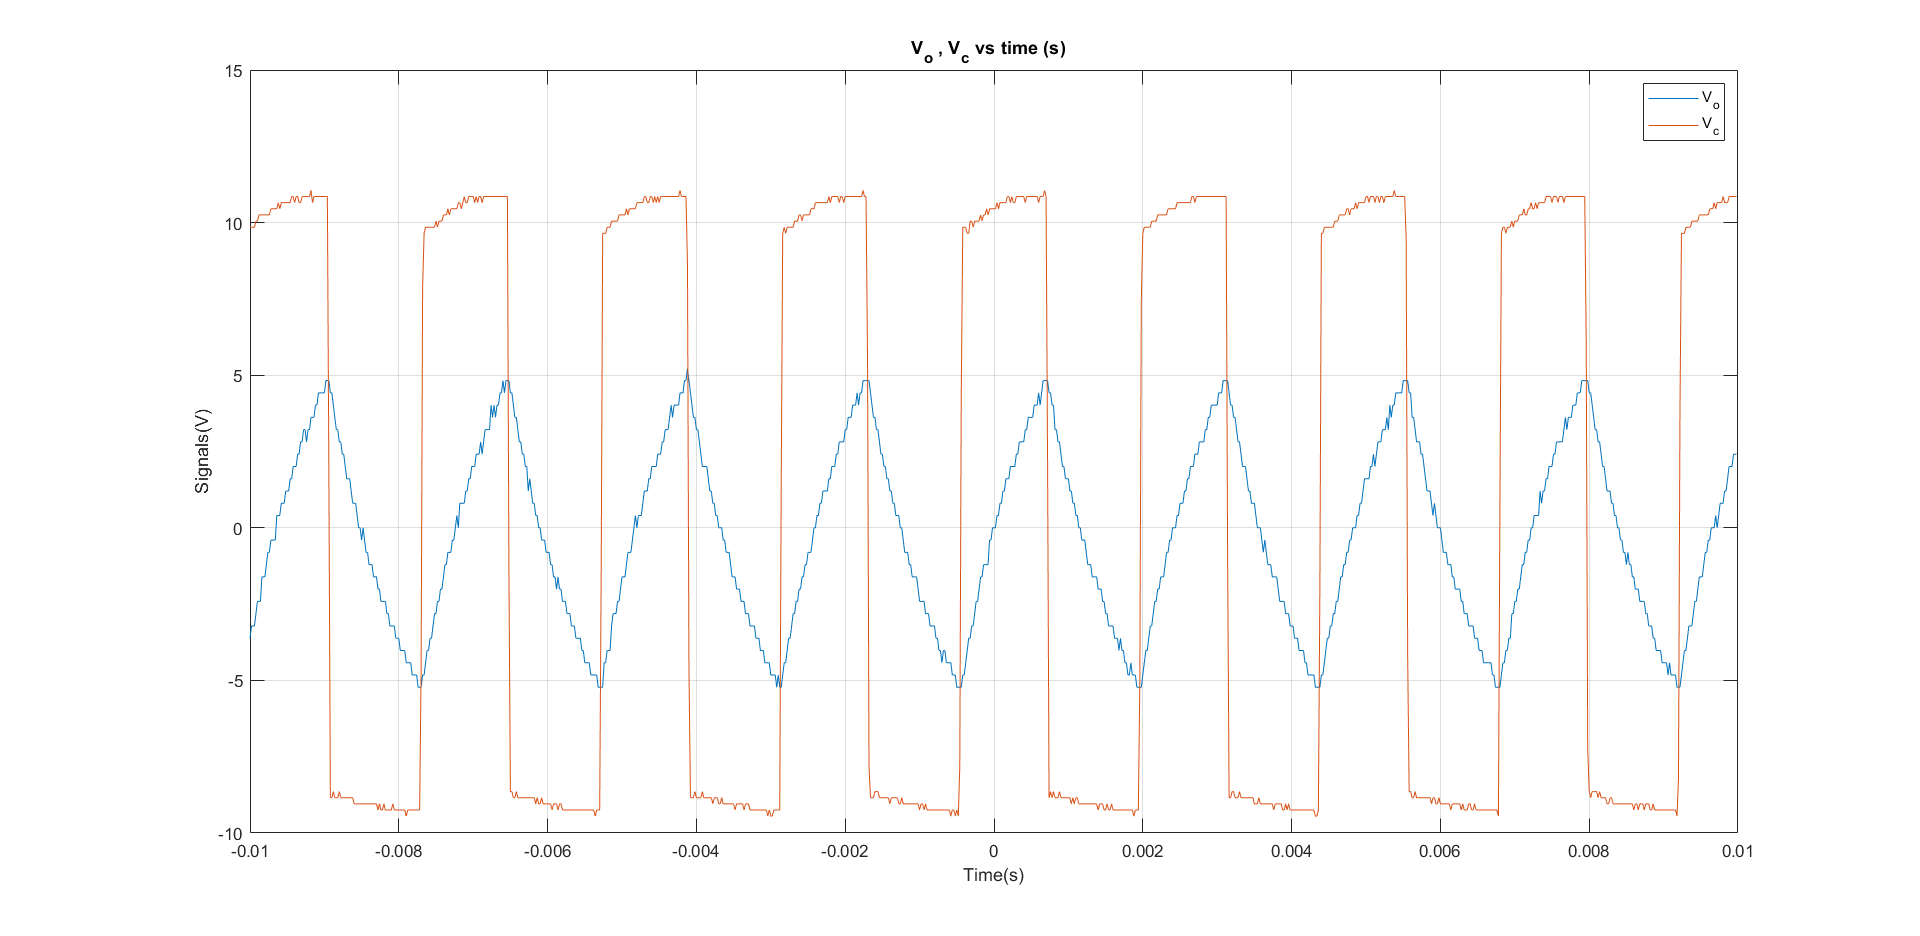
\includegraphics[width=1\textwidth]{3c_1_new.png}
   \caption{\(V_{c}\) , \(V_{in}\) vs time (s) }
\end{figure}
The result shows that the capacitor behaves like a signal generator that supplies a sawtooth-like signal. Different than the previous part, the measured frequency is found as approximately "413 Hz". The non-inverting operational amplifier configuration amplifies the signal supplied by the capacitor, and the output can be observed saturated. We can observe that the frequency of the signal supplied by the capacitor depends on the resistance connected to it. 

\subsection{Step 4}
In this step, the darkness sensor circuit given in Figure 22 is constructed.
\begin{figure}[H]
	\centering
   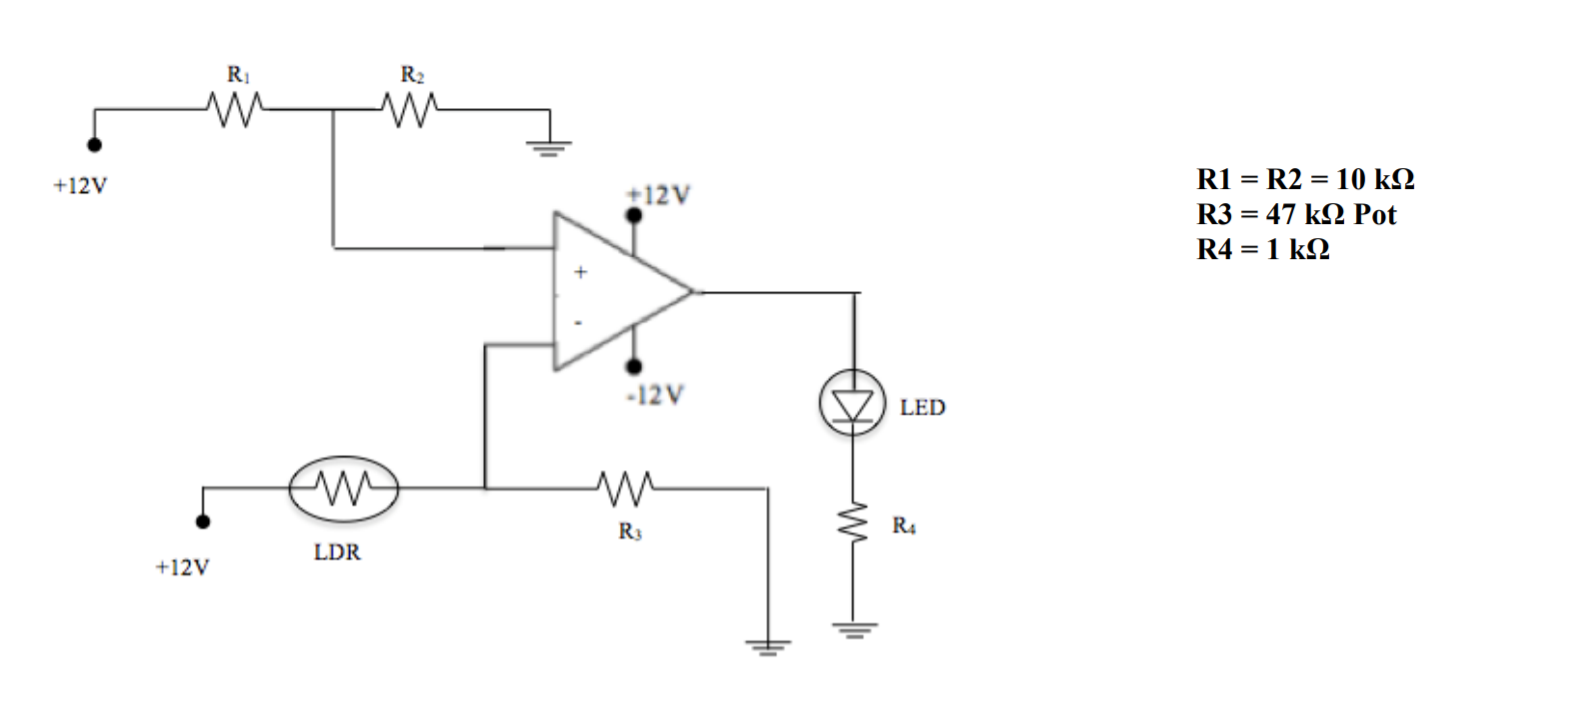
\includegraphics[width=1\textwidth]{darkness.png}
   \caption{Circuit schematic for Step 4}
\end{figure}
\subsubsection{a)}
The circuit is an example of a comparator; the opamp compares the voltage between its inverting and non-inverting terminals. At the non-inverting terminal, 6 Volts is supplied with a voltage divider setup. A voltage divider setup is constructed via an LDR and pot at the inverting terminal. When the LDR is in the dark, the led is on, so the system senses the darkness.
\subsubsection{b)}
For the , the lightness sensor proposed circuit given in Figure 23 is set. 
\begin{figure}[H]
	\centering
   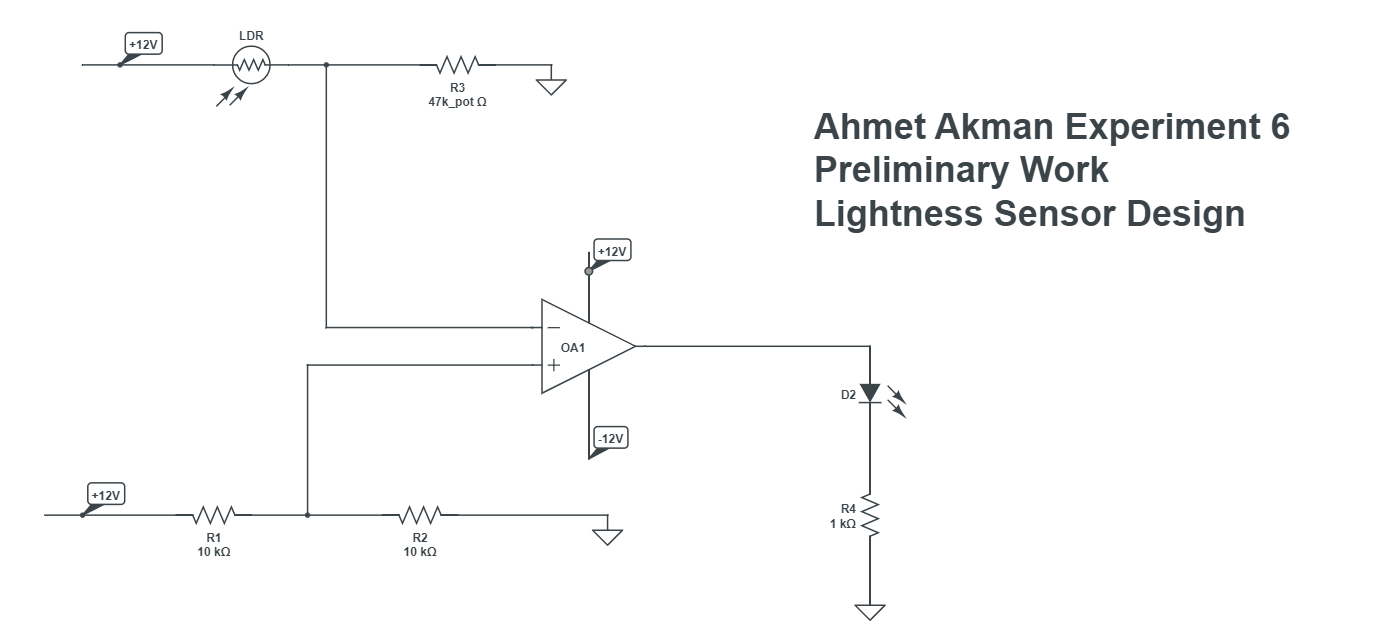
\includegraphics[width=1\textwidth]{lightness.png}
   \caption{Lightness sensor circuit schematic for Step 4 part b}
\end{figure}
The circuit is an example of a comparator; the opamp compares the voltage between its inverting and non-inverting terminals. At the inverting terminal, 6 Volts is supplied with a voltage divider setup. At the non-inverting terminal, a voltage divider setup is constructed via an LDR and pot. When the LDR is getting sufficient light, the led is on, so the system senses the lightness. The system can be tuned by adjusting the pot.
\subsubsection{c)}
The only difference between darkness and the lightness sensor is the terminals of the opamp are swapped. So the result of the comparison also swapped. This means the comparison reference is the only difference, and the polarity of the output determines whether led is on or off.
\subsection{Step 5}
In this step the circuit in Figure 24 is constructed.
\begin{figure}[H]
	\centering
   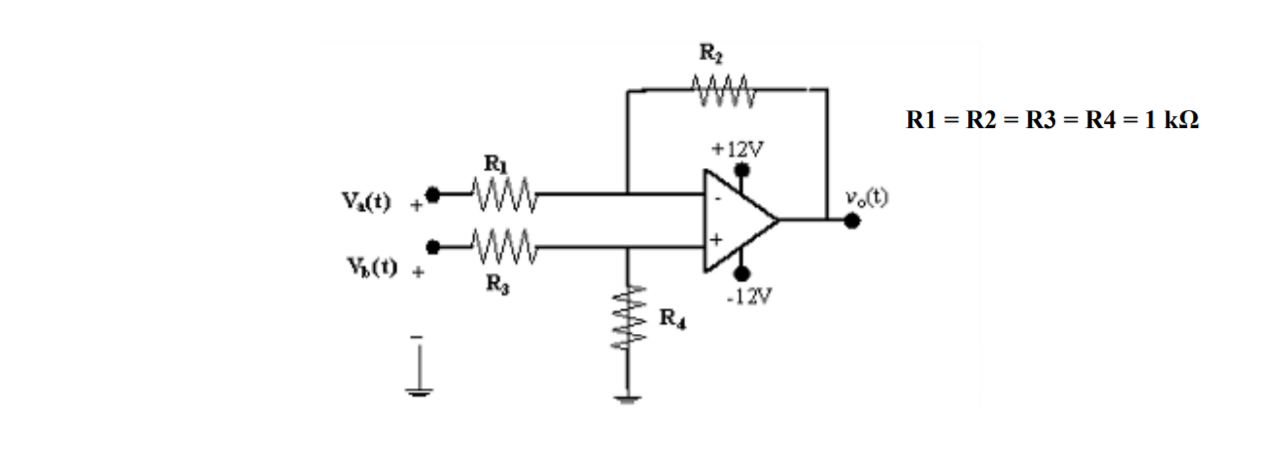
\includegraphics[width=1\textwidth]{circuit_6.png}
   \caption{Difference amplifier circuit schematic for Step 5}
\end{figure}
In order to supply two different signals with one signal generator, voltage is divided with three 1k\(\Omega\) resistors. Then to prevent voltage drop and let the voltage divider work properly, a buffer circuit is used, as given in Figure 25.
\begin{figure}[H]
	\centering
   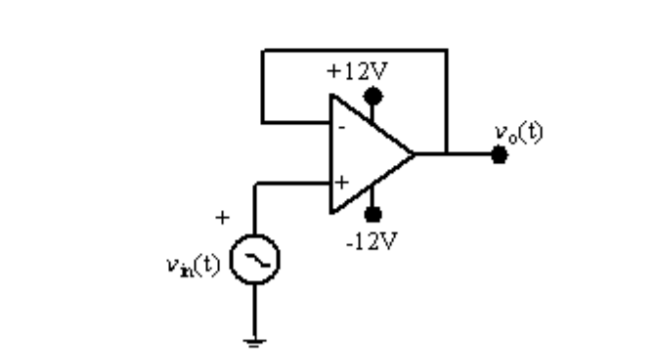
\includegraphics[width=1\textwidth]{buffer.png}
   \caption{Buffer circuit schematic for Step 5}
\end{figure}
So the \(V_a(t)\) = 3\(V_b(t)\) = \(4.5 sin(1000\pi t)\) signals are supplied to the circuit succesfully.
As a result, the input and output waveforms are plotted in MATLAB, given in Figure 26.
\begin{figure}[H]
	\centering
   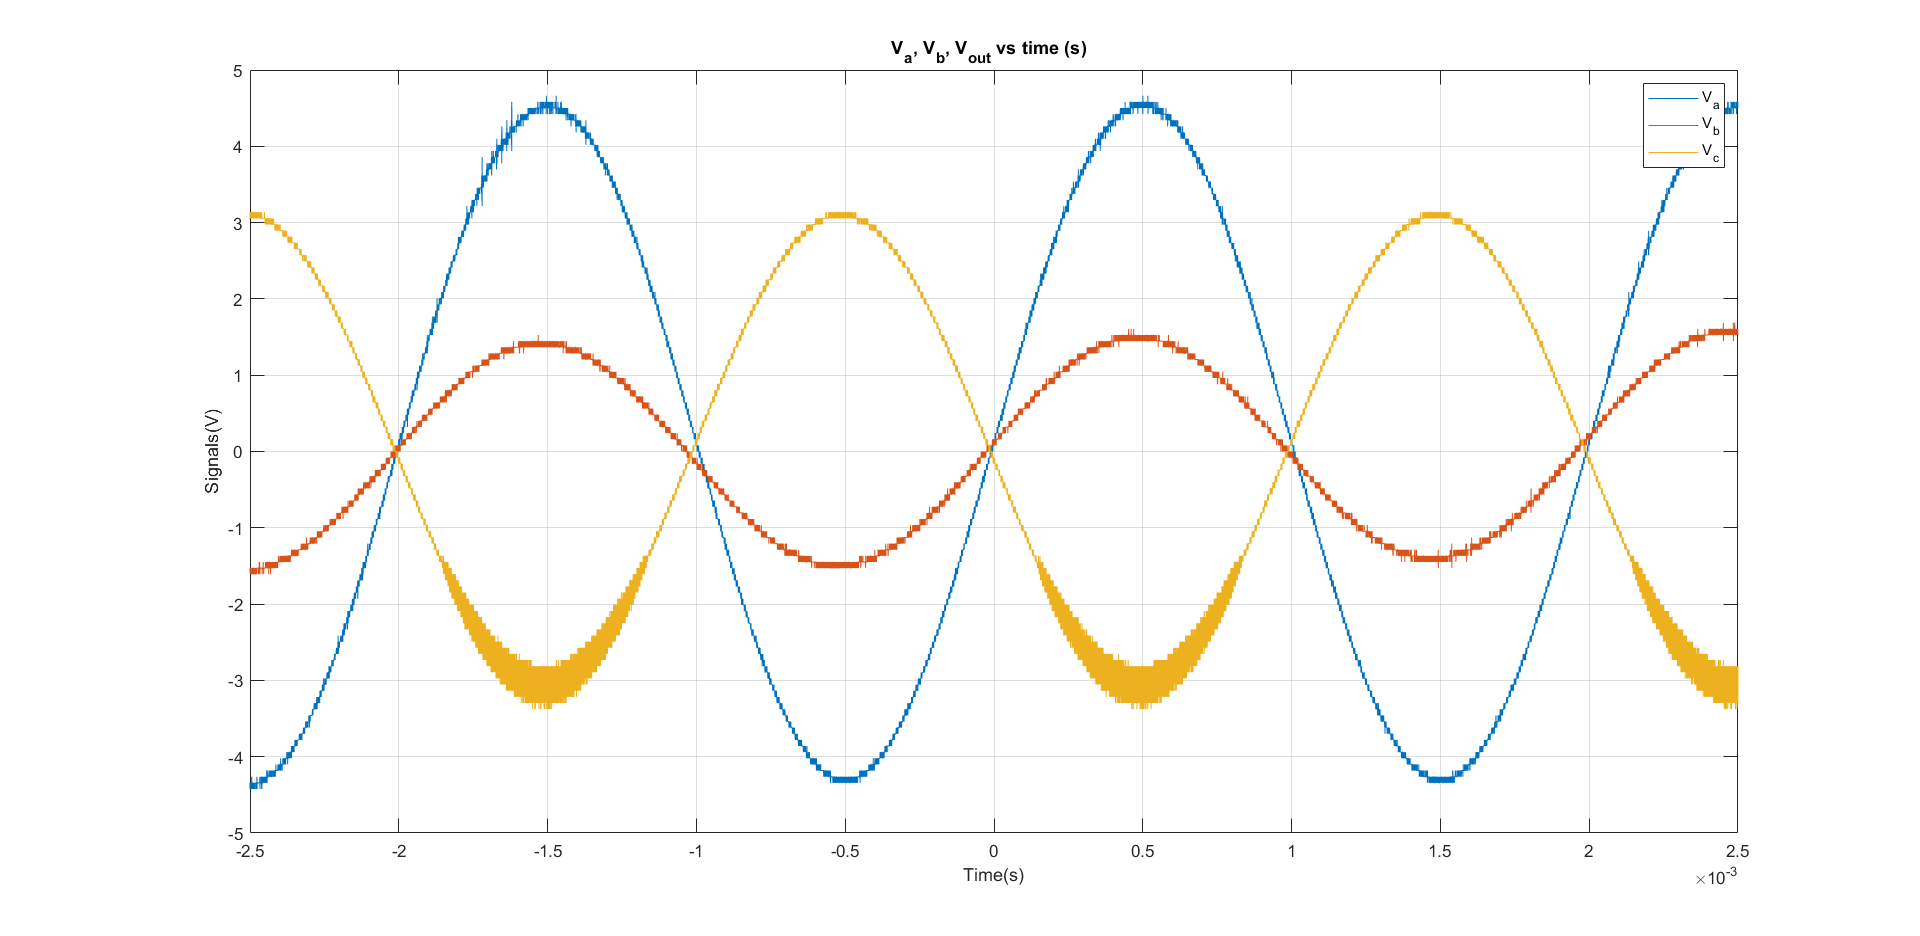
\includegraphics[width=1\textwidth]{5.png}
   \caption{\(V_{a}\), \(V_{b}\) , \(V_{o}\) vs time (s)}
\end{figure}
It can be stated that the resulting signal is the inverted version of the difference of the \(V_a\) and \(V_b\), whose amplitude is equal to approximately "3 Volts". Also, since the amplifier is set to invert, the resulting signal has the phase difference of \(\pi \) radians with respect to the \(V_a\) and \(V_b\). 
\section{Conclusion}
In conclusion, in experiment 6, "Operational Amplifiers-II," as students, we have learned how various functional circuit setups of Op-Amps can be constructed. Preliminary laboratory work is done via simulations of the Op-Amp circuits in an LTSpice environment and by hand calculations. As students, we have observed how the amplifying job can be done in two-stage and its advantages. We have seen the effect of non-linear feedback on the Op-Amp setup. The characteristics of the negative resistance converter are observed. Also, implementing darkness and lightness sensors has experienced a real-life design approach. Lastly, a difference amplifier circuit is set, and the characteristics are observed with measurements. To sum up, in this experiment, as students, we have experimented with how different kinds of operational amplifier circuits operate. 
\section*{Appendix I}
Total time spent on/during:
\begin{itemize}
	\item Pre-lab preparation: 6.5 hours (including the preliminary work and simulations) 
	\item Experimental work: 2 hours (hours spent in lab)
	\item Report writing: 6 hours 
\end{itemize}
\section*{Appendix II}
The outputs of the simulations are fetched from LTSpice and plotted in MATLAB.
%++++++++++++++++++++++++++++++++++++++++
% References section will be created automatically 
% with inclusion of "thebibliography" environment
% as it shown below. See text starting with line
% \begin{thebibliography}{99}
% Note: with this approach it is YOUR responsibility to put them in order
% of appearance.

%\begin{thebibliography}{99}

%https://tr.overleaf.com/latex/templates/sample-lab-report-for-u-of-r-phys-349/pgsyqngcyjxk

%\end{thebibliography}


\end{document}


\begin{table}[H]
	\begin{center}
		\caption{Resistance reading by color code convention.}
		\vspace{2mm}
		\begin{tabular}{||c | c | c||} 
		 \hline
		 Color Order & Value & Tolerance \\ [0.5ex] 
		 \hline\hline
		 Brown / Black / Red / Gold & 1k\( \Omega \) & \( \% \) 5  \\ 
		 \hline
		 Yellow / Violet / Red / Gold & 4.7k\( \Omega \) & \( \% \) 5   \\
		 \hline
		 Brown / Grey / Orange / Gold & 18k\( \Omega \) & \( \% \) 5  \\ [1ex] 
		 \hline
		\end{tabular}
	\end{center}
	\end{table}

	\begin{figure}[H]
 		\centering
		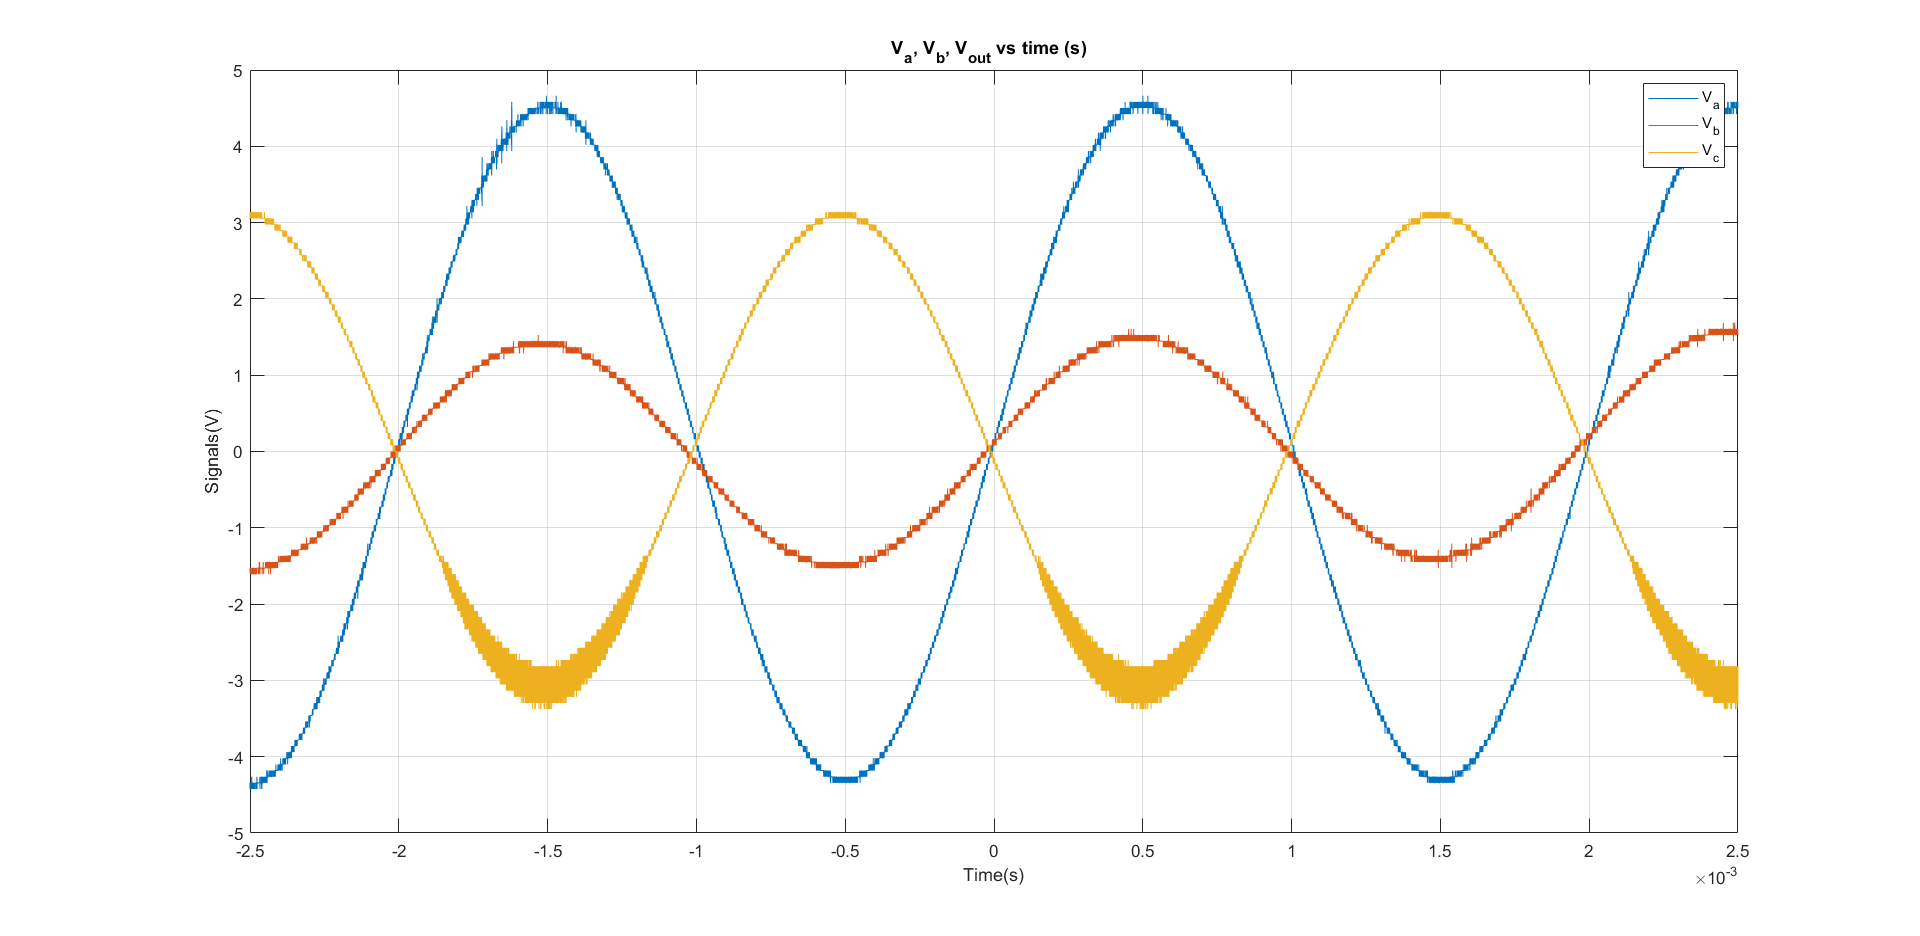
\includegraphics[width=0.6\textwidth]{5.png}
		\caption{Circuit schematic for the step 5}
	\end{figure} 

	\begin{figure}[htp] \centering{
		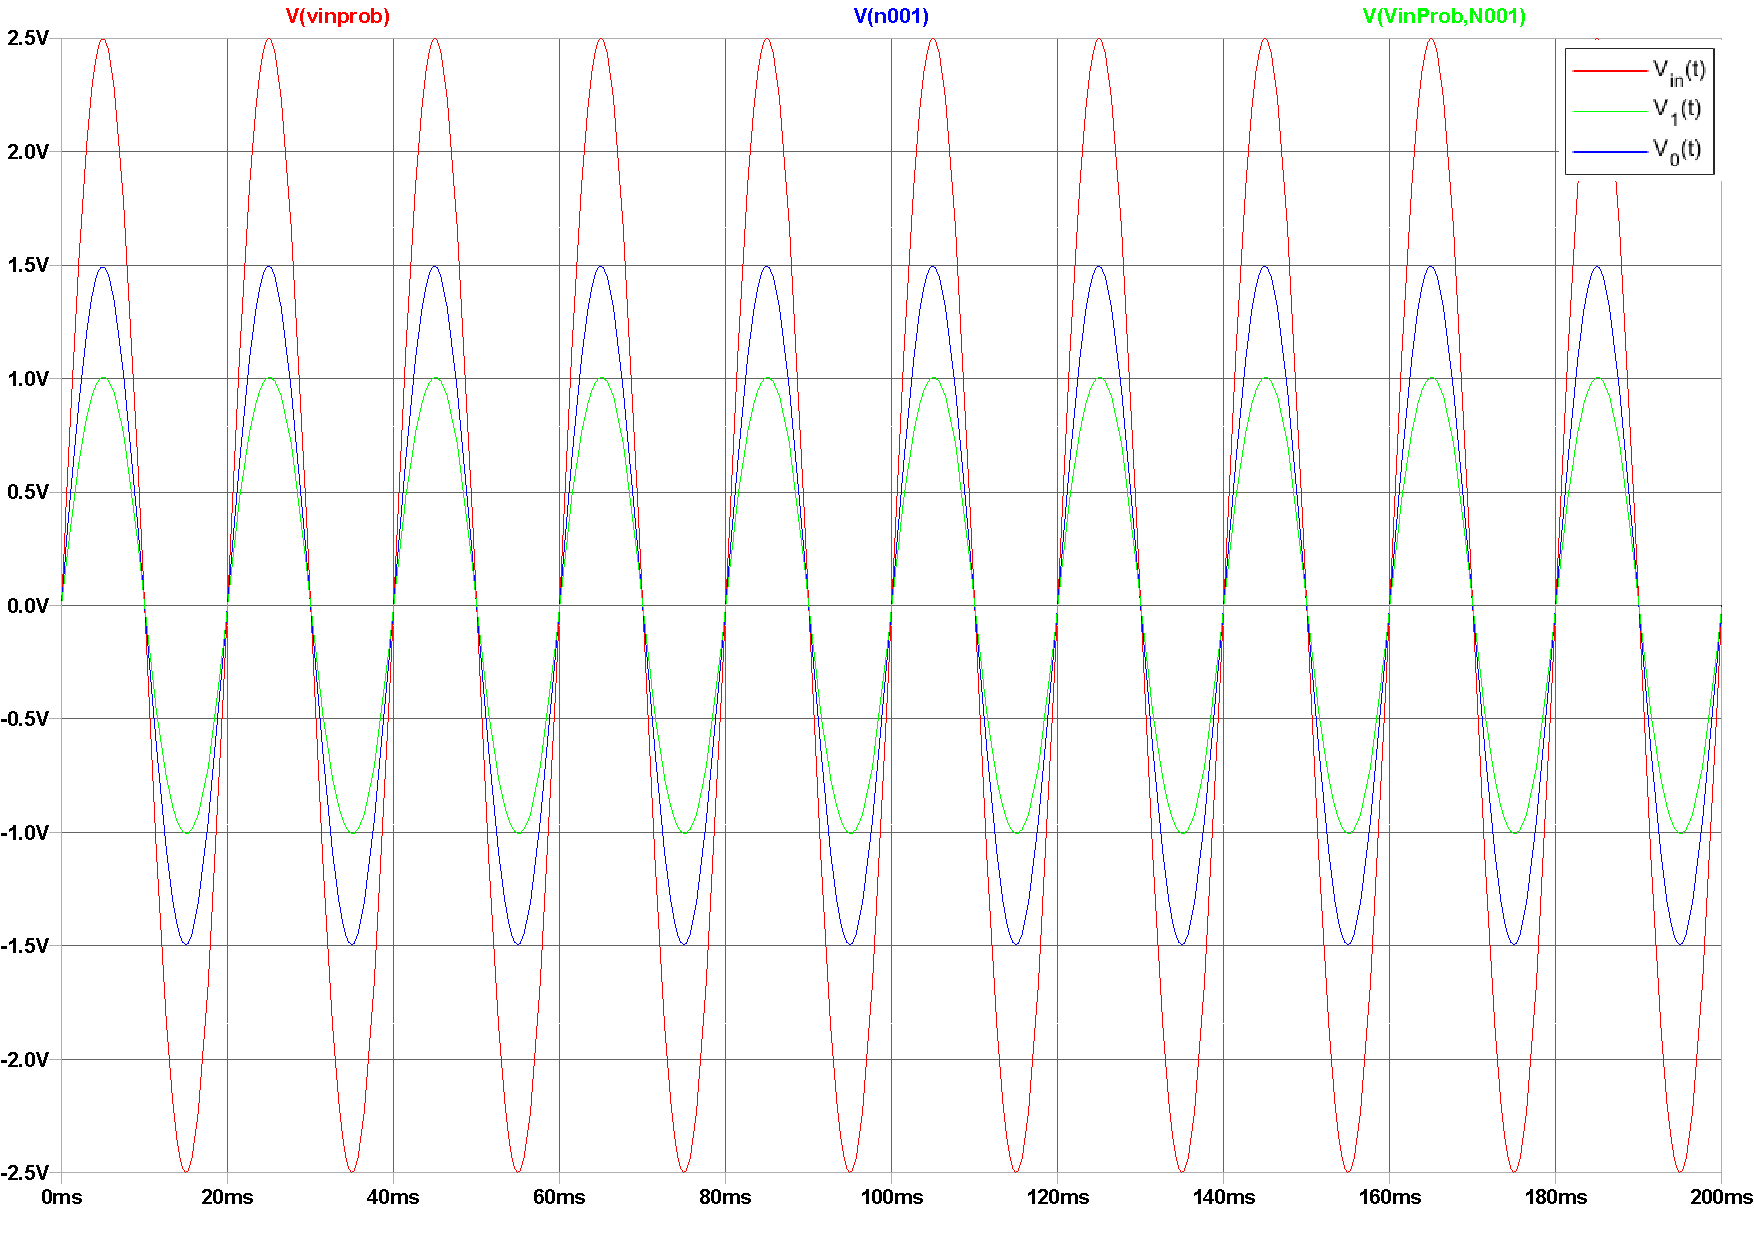
\includegraphics[scale=0.25]{2a_plot.pdf}}
		\caption{Experiment 2}
\end{figure}
	